\section{Experiments}\label{sec:experiment}
We experimentally evaluated the performance and quality of our methodology (heuristic algorithm in \cref{subsec:heuristics}), and compared it against the exhaustive approach in~\cref{sec:nphard}. In the following,
\cref{subsec:experiments_infrastructure} presents the simulator and testing infrastructure adopted in our experiments;
%, as well as the complete experimental settings;
\cref{subsec:experiments_performance} analyses the performance of our solution in terms of execution time; \cref{subsec:experiments_quality} presents the quality of our heuristic algorithm in generating of the best pipeline instance according to the metrics $M_J$ and $M_{JSD}$ in \cref{subsec:metrics}.

\subsection{Testing Infrastructure and Experimental Settings}\label{subsec:experiments_infrastructure}
Our testing infrastructure is a Swift-based simulator of a service-based ecosystem, including service execution, comparison, and composition. The simulator first defines the pipeline template as a sequence of vertices, with $l$ the length of the pipeline template) and defines the size \windowsize\ of the sliding window, such that \windowsize$\leq$$l$. We recall that alternative vertices are modeled in different pipeline templates, while parallel vertices are not considered since they only add a fixed execution time that is negligible and do not affect the performance and quality of our approach. Each vertex is associated with a (set of) policy that applies a filtering transformation that remove a given percentage of data.
% Our testing infrastructure is a Swift-based simulator of a service-based ecosystem, including service execution, comparison, and composition. The simulator first defines the pipeline template as a sequence of vertices in the range 3$-$7 (the length $l$ of the pipeline template) and defines the size \windowsize\ of the sliding window, such that \windowsize$<$$l$. We recall that alternative vertices are modeled in different pipeline templates, while parallel vertices are not considered since they only add a fixed execution time that is negligible and do not affect the performance and quality of our approach. Each vertex is associated with a (set of) policy that applies a filtering transformation that either remove a percentage of data in $[0.5,0.8]$ (\average) or in $[0.20,1]$ (\wide).
% % \begin{enumerate*}[label=\textit{\roman*})]
% %   \item \average: data removal percentage within $[0.5,0.8]$.
% %   \item \wide:    data removal percentage within
% % \end{enumerate*}

The simulator then starts the instantiation process as shown in Figure~\ref{fig:execution_example}. At each step $i$, it selects the subset \{\vi{i},$\ldots$,$v_{\windowsize+i-1}$\} of vertices with their corresponding candidate services, and generates all possible service combinations. For each combination, the simulator calculates a given metric $M$ and selects the service that instantiates \vi{i} from the optimal combination according to $M$. The window is shifted step 1 (i.e., $i$=$i$+1) and the instantiation process restart. When the sliding window reach the end of the pipeline template, that is, $v_{\windowsize+i-1}$$=$$\vi{l}$, the simulator computes the optimal service combination and instantiates the remaining vertices with the corresponding services.

We note that a hash function randomly simulates the natural interdependence between services, modeling a data removal on one service that might impact another one. \hl{LA SPECIFICHIAMO UN PO' MEGLIO?} %By assigning weights to the services using this function, the system aims to reflect the interconnected dynamics among the services.

%The simulator is used to assess the performance and quality of our sliding window heuristic in Section \ref{sec:heuristics} for the generation of the best pipeline instance (Section \ref{sec:instance}).
% Performance measures the heuristics execution time in different settings, while quality compares the results provided by our heuristics in terms of selected services with the optimal solution retrieved using the exhaustive approach.
%We note that the exhaustive approach generates the best pipeline instance by executing all possible combinations of candidate services.
%The emulator simplifies the execution of the service composition by removing the service selection phase, which is not relevant for the purpose of the experiment.
Our experiments have been run on a virtual machine equipped with a Intel(R) Xeon(R) CPU E5-2620 v4 @ 2.10GHz CPU and 32GB RAM.
Each experiment was repeated 10 times and the results averaged to improve the reliability of findings.

\begin{figure}[!t]
  \centering
  \resizebox{\columnwidth}{!}{%
    \begin{tikzpicture}[framed]

      \node[draw, circle, fill=gray!20,minimum width=1.2cm] (v1) at (1,5.2) {$\vi{1}$};
      \node[draw, circle, fill=gray!20,minimum width=1.2cm] (v2) at (3,5.2) {$\vi{2}$};
      \node[draw, circle, fill=gray!20,minimum width=1.2cm] (v3) at (5,5.2) {$\vi{3}$};
      \node[draw, circle, fill=gray!20,minimum width=1.2cm] (v4) at (7,5.2) {$\vi{4}$};
      \node[draw, circle, fill=gray!20,minimum width=1.2cm] (v5) at (9,5.2) {$\vi{5}$};
      \node[above, shift=({0,0.5}) ] at (v3.north)  {Sliding Window};

      \node[draw, rectangle,fill=red!20] (s41) at (1,3.4) {$\sii{1}$};
      \node[draw, rectangle, fill=green!20] (s42) at (1,1.7) {$\sii{2}$};
      \node[draw, rectangle, fill=red!20] (s43) at (1,0) {$\sii{3}$};

      \node[draw, rectangle] (s1) at (3,3.4) {$\sii{11}$};
      \node[draw, rectangle] (s2) at (3,1.7) {$\sii{12}$};
      \node[draw, rectangle] (s3) at (3,0) {$\sii{13}$};

      \node[draw, rectangle] (s11) at (5,3.4) {$\sii{21}$};
      \node[draw, rectangle] (s12) at (5,1.7) {$\sii{22}$};
      \node[draw, rectangle] (s13) at (5,0) {$\sii{23}$};

      \node[draw, rectangle] (s21) at (7,3.4) {$\sii{31}$};
      \node[draw, rectangle] (s22) at (7,1.7) {$\sii{32}$};
      \node[draw, rectangle] (s23) at (7,0) {$\sii{33}$};

      \node[draw, rectangle] (s31) at (9,3.4) {$\sii{41}$};
      \node[draw, rectangle] (s32) at (9,1.7) {$\sii{42}$};
      \node[draw, rectangle] (s33) at (9,0) {$\sii{43}$};


      % \draw[->] (node2) -- (node3);
      \draw[->] (s42) -- (s1);
      \draw[->] (s42) -- (s2);
      \draw[->] (s42) -- (s3);

      \draw[->] (s1) -- (s11);
      \draw[->] (s1) -- (s12);
      \draw[->] (s1) -- (s13);

      \draw[->,dashdotted] (s2) -- (s11);
      \draw[->,dashdotted] (s2) -- (s12);
      \draw[->,dashdotted] (s2) -- (s13);

      \draw[->,dashed] (s3) -- (s11);
      \draw[->,dashed] (s3) -- (s12);
      \draw[->,dashed] (s3) -- (s13);


      \draw[->] (s11) -- (s21);
      \draw[->] (s11) -- (s22);
      \draw[->] (s11) -- (s23);

      \draw[->,dashdotted] (s12) -- (s21);
      \draw[->,dashdotted] (s12) -- (s22);
      \draw[->,dashdotted] (s12) -- (s23);

      \draw[->,dashed] (s13) -- (s21);
      \draw[->,dashed] (s13) -- (s22);
      \draw[->,dashed] (s13) -- (s23);

      \draw[->] (v1) -- (v2);
      \draw[->] (v2) -- (v3);
      \draw[->] (v3) -- (v4);
      \draw[->] (v4) -- (v5);


      \begin{scope}[on background layer]
        \draw[thick, dashed, fill=red!10, opacity=0.5]
        ([shift={(-0.5,0.5)}]s1.north west) rectangle ([shift={(0.5,-0.5)}]s23.south east);



      \end{scope}
      \begin{scope}[on background layer]
        \draw[thick, dashed, fill=red!10, opacity=0.5]
        ([shift={(-0.5,0.5)}]v2.north west) rectangle ([shift={(0.5,-0.5)}]v4.south east);

      \end{scope}


    \end{tikzpicture}
  }
  \caption{Execution example}
  \label{fig:execution_example}
\end{figure}

\subsection{Perfomance}\label{subsec:experiments_performance}
% \subsection{performance}
% \begin{itemize}
%   \item Finestra scorrevole da 1 a N=Nodi
%   \item Servizi 5 a 20 passo 5 + 50??
%   \item
% \end{itemize}
% \subsection{Metriche/Euristiche}
We first measured the performance (execution time) of our exhaustive and heuristic solutions. To this aim, we varied the number of vertices from 2 to 5 (step 1) and the number of services per vertex from 2 to 6 (step 1). \cref{fig:perf_exhaustive} presents our results for the exhaustive solution, showing an exponential trend in the execution time. We can observe that, as the number of vertices increases, the execution time grows exponentially. Execution times for up to 5 vertices and 6 services were computed, while the remaining data points were obtained through interpolation.\hl{QUALI SONO INTERPOLATI? 5 E 6 SONO TUTTI I CASI.}
%Subsequently, the logical extension of this empirical inquiry involves evaluating the execution time efficiency attributable to the implementation of the sliding window heuristic.

We then evaluated our heuristic and measured its performance (execution time) varying the window size \windowsize\ from X to Y (step 1). \cref{fig:perf_window} (log scale) presents our results for the heuristic solution. We can observe a substantial reduction in execution time, with the heuristic always able to produce an instance in less than \hl{TO ADD}.\hl{NON VEDO LA FIGURA.}
\begin{figure}[htb!]
  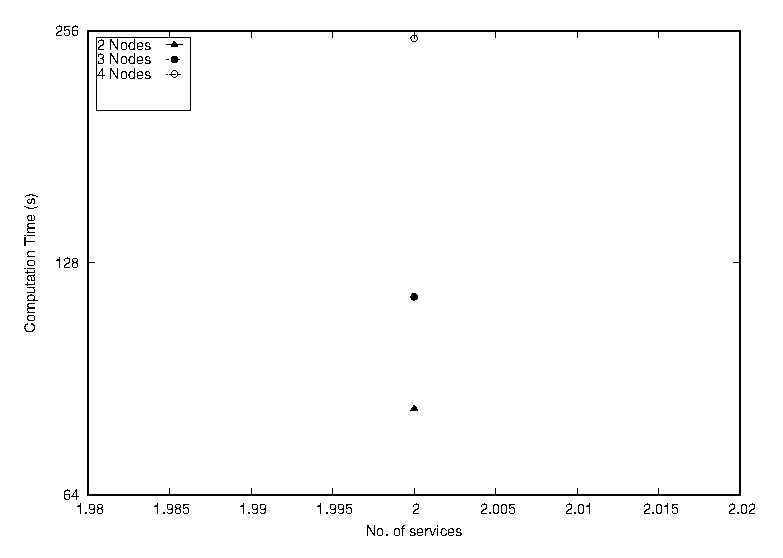
\includegraphics[width=0.95\columnwidth]{graphs/exhaustive_performance.eps}
  \caption{Exhaustive execution time evaluation. The x-axis represents the number of services, while the y-axis represents the execution time in seconds. The execution time is expressed both in linear and logarithmic scales.}
  \label{fig:perf_exhaustive}
\end{figure}


\subsection{Quality}\label{subsec:experiments_quality}
We finally evaluated the quality of our heuristic with different \windowsize\ comparing, where possible, its results with the optimal solution retrieved by executing the exhaustive approach. %The latter is executed with window size equals to the number of vertices in the pipeline template, and provides the best, among all possible, solutions.
The quality of the heuristic was then calculated as the ratio between the value of metric $M$ retrieved by the heuristic and the one obtained by the exhaustive approach.


We run our experiments varying: \emph{i)} the length $l$ of the pipeline template in [3,7], that is, the number of vertices composed in a sequence, \emph{ii)} the window size \windowsize\ in [1,$l$], and \emph{iii)} the number of candidate services for each vertex in the pipeline template in [2, 7]. Each vertex is associated with a (set of) policy that applies a filtering transformation that either remove a percentage of data in $[0.5,0.8]$ (\average) or in $[0.20,1]$ (\wide).



\cref{fig:quality_window_average_perce,fig:quality_window_perce_wide} present our results with metric $M_J$ in \cref{subsec:metrics} for settings \wide and \average, respectively.
In general, we observe that the quality of our heuristic approach increases as the window size increases, providing a quality comparable to the exhaustive approach when the window size \windowsize\ approaches the length $l$ of the pipeline template.

When considering setting \wide, the greedy approach (\windowsize=1) provides good results on average (from X to Y), it shows substantial oscillations, for instance, varying the quality between 0.882 and 0.970 for 3 vertices, 0.810 and 0.942 for 4 vertices, 0.580 and 0.853 for 5 vertices, 0.682 and 0.943 for 6 vertices, 0.596 and 0.821 for 7 vertices. This same trends emerge when the window size is less than $l$/2, while it starts approaching the optimum when the window size is higher than $l$/2. For instance, when \windowsize=$l$-1, the quality varis between 0.957 and 1.0 for 3 vertices, 0.982 and 1.0 for 4 vertices, 0.986 and 0.998 for 5 vertices, 0.977 and 1.0 for 6 vertices, 0.996 and 1.0 for 7 vertices.

When considering setting \average, the greedy approach (\windowsize=1) provides good results on average (from X to Y), it shows substantial oscillations, for instance, varying the quality between 0.927 and 0.978 for 3 vertices, 0.903 and 0.962 for 4 vertices, 0.840 and 0.915 for 5 vertices, 0.815 and 0.934 for 6 vertices, 0.721 and 0.935 for 7 vertices. This same trends emerge when the window size is less than $l$/2, while it starts approaching the optimum when the window size is higher than $l$/2. For instance, when \windowsize=$l$-1, the quality varis between 0.980 and 1.0 for 3 vertices, 0.978 and 1.0 for 4 vertices, 0.954 and 1 for 5 vertices, 0.987 and 1.0 for 6 vertices, 0.990 and 1.0 for 7 vertices.
% \hl{RIVEDI DA QUA COME SOPRA FINO A...}

% In a configuration employing a \wide setting with three nodes, the average quality ratio for a window size of one is 0.93, with a standard deviation of 0.02; for a window size of two, it is 0.98 with a standard deviation of 0.01. When the number of nodes is increased to four, the average quality ratios observed are 0.88 for a window size of one (standard deviation = 0.04), 0.96 for a window size of two (standard deviation = 0.02), and 0.99 for a window size of three. Further increasing the node count to five yields average quality ratios of 0.76 for a window size of one (standard deviation = 0.09), 0.90 for a window size of two (standard deviation = 0.04), with further increments in window sizes of three and four maintaining standard deviations of 0.01.
% For six nodes, the average quality ratios are as follows: 0.78 for a window size of one (standard deviation = 0.09); 0.87 for a window size of two (standard deviation = 0.04); 0.95 for a window size of three (standard deviation = 0.02); 0.97 for a window size of four (standard deviation = 0.02); and 0.99 for a window size of five. Notably, the range of quality ratios (maximum-minimum) narrows as the window size increases, from 0.261 for a window size of one to 0.14 for a window size of two, and further to 0.02 for a window size of five.
% In a seven-node configuration, the average quality ratios are as follows: 0.73 for a window size of one (standard deviation = 0.08); 0.87 for a window size of two (standard deviation = 0.08); 0.95 for a window size of three (standard deviation = 0.02); 0.96 for a window size of four (standard deviation = 0.02); and 0.99 for both window sizes of five and six (standard deviation = 0.02 each).

% In an \average setting with three nodes, the average quality ratios are 0.95 for a window size of one, with a standard deviation of 0.017, and 0.99 for a window size of two, with a standard deviation of 0.006. Expanding to four nodes, the quality ratios observed are 0.93 for a window size of one (standard deviation = 0.019), 0.97 for a window size of two (standard deviation = 0.006), and 0.99 for a window size of three (standard deviation = 0.007). Increasing the node count to five yields average quality ratios of 0.88 for a window size of one (standard deviation = 0.02), 0.93 for a window size of two (standard deviation = 0.03), 0.97 for a window size of three (standard deviation = 0.015), and 0.98 for a window size of four (standard deviation = 0.016).
% For six nodes, the quality ratios are as follows: 0.87 for a window size of one (standard deviation = 0.047), 0.92 for a window size of two (standard deviation = 0.058), 0.96 for a window size of three (standard deviation = 0.021), 0.97 for a window size of four (standard deviation = 0.014), and 0.99 for a window size of five (standard deviation = 0.004). For seven nodes, the respective quality ratios are 0.83 for a window size of one (standard deviation = 0.068), 0.92 for a window size of two (standard deviation = 0.030), 0.98 for both window sizes of three and four (standard deviation = 0.007 and 0.017), and 0.99 for window sizes of five and six (standard deviation = 0.006 and 0.004).

\cref{fig:quality_window_wide_qualitative,fig:quality_window_average_qualitative} display the outcomes assessed metric $M_{JSD}$ in \cref{subsec:metrics} for settings \wide and \average, respectively.

When considering setting \wide, the greedy approach (\windowsize=1) provides good results on average (from X to Y), it shows substantial oscillations, for instance, varying the quality between 0.954 and 0.993 for 3 vertices, 0.939 and 0.993 for 4 vertices, 0.899 and 0.960 for 5 vertices, 0.878 and 0.949 for 6 vertices, 0.870 and 0.914 for 7 vertices. This same trends emerge when the window size is less than $l$/2, while it starts approaching the optimum when the window size is higher than $l$/2. For instance, when \windowsize=$l$-1, the quality varis between  0.991 and  1,0 for 3 vertices, 0.989 and 1.0 for 4 vertices, 0.994 and 1.0 for 5 vertices, 0.993 and 1.0 for 6 vertices, 0.997 and 1.0 for 7 vertices.


When considering setting \average, the greedy approach (\windowsize=1) provides good results on average (from X to Y), it shows substantial oscillations, for instance, varying the quality between 0.981 and 0.994 for 3 vertices, 0.957 and 0.991 for 4 vertices, 0.973 and 0.984 for 5 vertices, 0.947 and 0.974 for 6 vertices, 0.925 and 0.981 for 7 vertices. This same trends emerge when the window size is less than $l$/2, while it starts approaching the optimum when the window size is higher than $l$/2. For instance, when \windowsize=$l$-1, the quality varis between  0.993 and  0.999 for 3 vertices, 0.997 and 1.0 for 4 vertices, 0.997 and 1.0 for 5 vertices, 0.996 and 1.0 for 6 vertices, 0.996 and 1.0 for 7 vertices.
% In a \wide setting with three nodes, average quality ratios were observed as 0.98 for a window size of one, with a standard deviation of 0.014, and 0.998 for a window size of two, with a standard deviation of 0.005. Increasing the node count to four, the quality ratios are 0.97 for a window size of one (standard deviation = 0.019), 0.99 for a window size of two (standard deviation = 0.004), and 0.996 for a window size of three (standard deviation = 0.004).

% For five nodes, the quality ratios extend as follows: 0.93 for a window size of one (standard deviation = 0.022), 0.97 for a window size of two (standard deviation = 0.015), 0.993 for a window size of three (standard deviation = 0.006), and 0.998 for a window size of four (standard deviation = 0.003). In a configuration with six nodes, the quality ratios are 0.92 for a window size of one (standard deviation = 0.028), 0.97 for a window size of two (standard deviation = 0.018), 0.995 for a window size of three (standard deviation = 0.004), 0.996 for a window size of four (standard deviation = 0.005), and 0.998 for a window size of five (standard deviation = 0.003).

% Finally, with seven nodes, the quality ratios are 0.90 for a window size of one (standard deviation = 0.016), 0.96 for a window size of two (standard deviation = 0.019), 0.97 for a window size of three (standard deviation = 0.010), 0.994 for a window size of four (standard deviation = 0.005), 0.997 for a window size of five (standard deviation = 0.003), and 0.999 for a window size of six (standard deviation = 0.003).

% In an \average setting with three nodes, the average quality ratios are 0.99 for a window size of one, with a standard deviation of 0.003, and 1.00 for a window size of two, with a standard deviation of 0.000. When the configuration includes four nodes and window sizes from one to three, the quality ratios are 0.98 (standard deviation = 0.010), 0.99 (standard deviation = 0.003), and 1.00 (standard deviation = 0.003).

% Expanding to five nodes, the quality ratios are 0.98 for a window size of one (standard deviation = 0.004), 0.99 for a window size of two (standard deviation = 0.003), 1.00 for both window sizes three and four (standard deviations = 0.004 and 0.000, respectively). In a configuration with six nodes and window sizes ranging from one to five, the quality ratios are 0.97 (standard deviation = 0.006), 0.98 (standard deviation = 0.003), and 1.00 for window sizes three through five (standard deviations = 0.000, 0.003, and 0.003).

% For seven nodes, with window sizes extending from one to six, the quality ratios are 0.96 (standard deviation = 0.019), 0.98 (standard deviation = 0.009), 0.99 for both window sizes three and four (standard deviation = 0.005), and 1.00 for window sizes five and six (standard deviations = 0.003 and 0.000).

% \hl{...FINO A QUI}

% We note that the benefit of an increasing window size can be appreciated with lower numbers, reaching a sort of saturation around the average length (e.g., window of length 6 with a 7-vertex pipeline) where the quality ratio overlaps. The only exception is for 6-vertex pipeline where the overapping starts with window size 2. However, this might be due to the specific setting and therefore does not generalize.
% %Thus because the heuristic has more services to choose from and can find a better combination.
% We also observe that, as the window size increase, the quality increase as well. This suggests that the heuristic performs better when it has a broader perspective of the data it is governing.
% It's worth noting that lower window sizes are more unstable, with the quality ratio varying significantly between different configuration while higher window sizes tend to stabilize the quality ratio across different configuration.


Finally, the data suggest that while larger window sizes generally lead to better performance, there might exist a point where the balance between window size and performance is optimized. Beyond this point, the incremental gains in metric values may not justify the additional computational resources or the complexity introduced by larger windows.
It's worth noting that lower window sizes are more unstable, with the quality ratio varying significantly between different configuration while higher window sizes tend to stabilize the quality ratio across different configuration.

The proposed heuristics show ability to approximate the results obtained via an exhaustive approach. However, to comprehensively understand the influence of dataset selection on the metrics' performance and ensure their robustness across diverse scenarios, a dedicated investigation is essential. This further research will validate the preliminary findings and provide a deeper insight into the applicability of the heuristics in various contexts.
\begin{figure*}[!htb]
  \centering
  \begin{subfigure}{0.33\textwidth}
    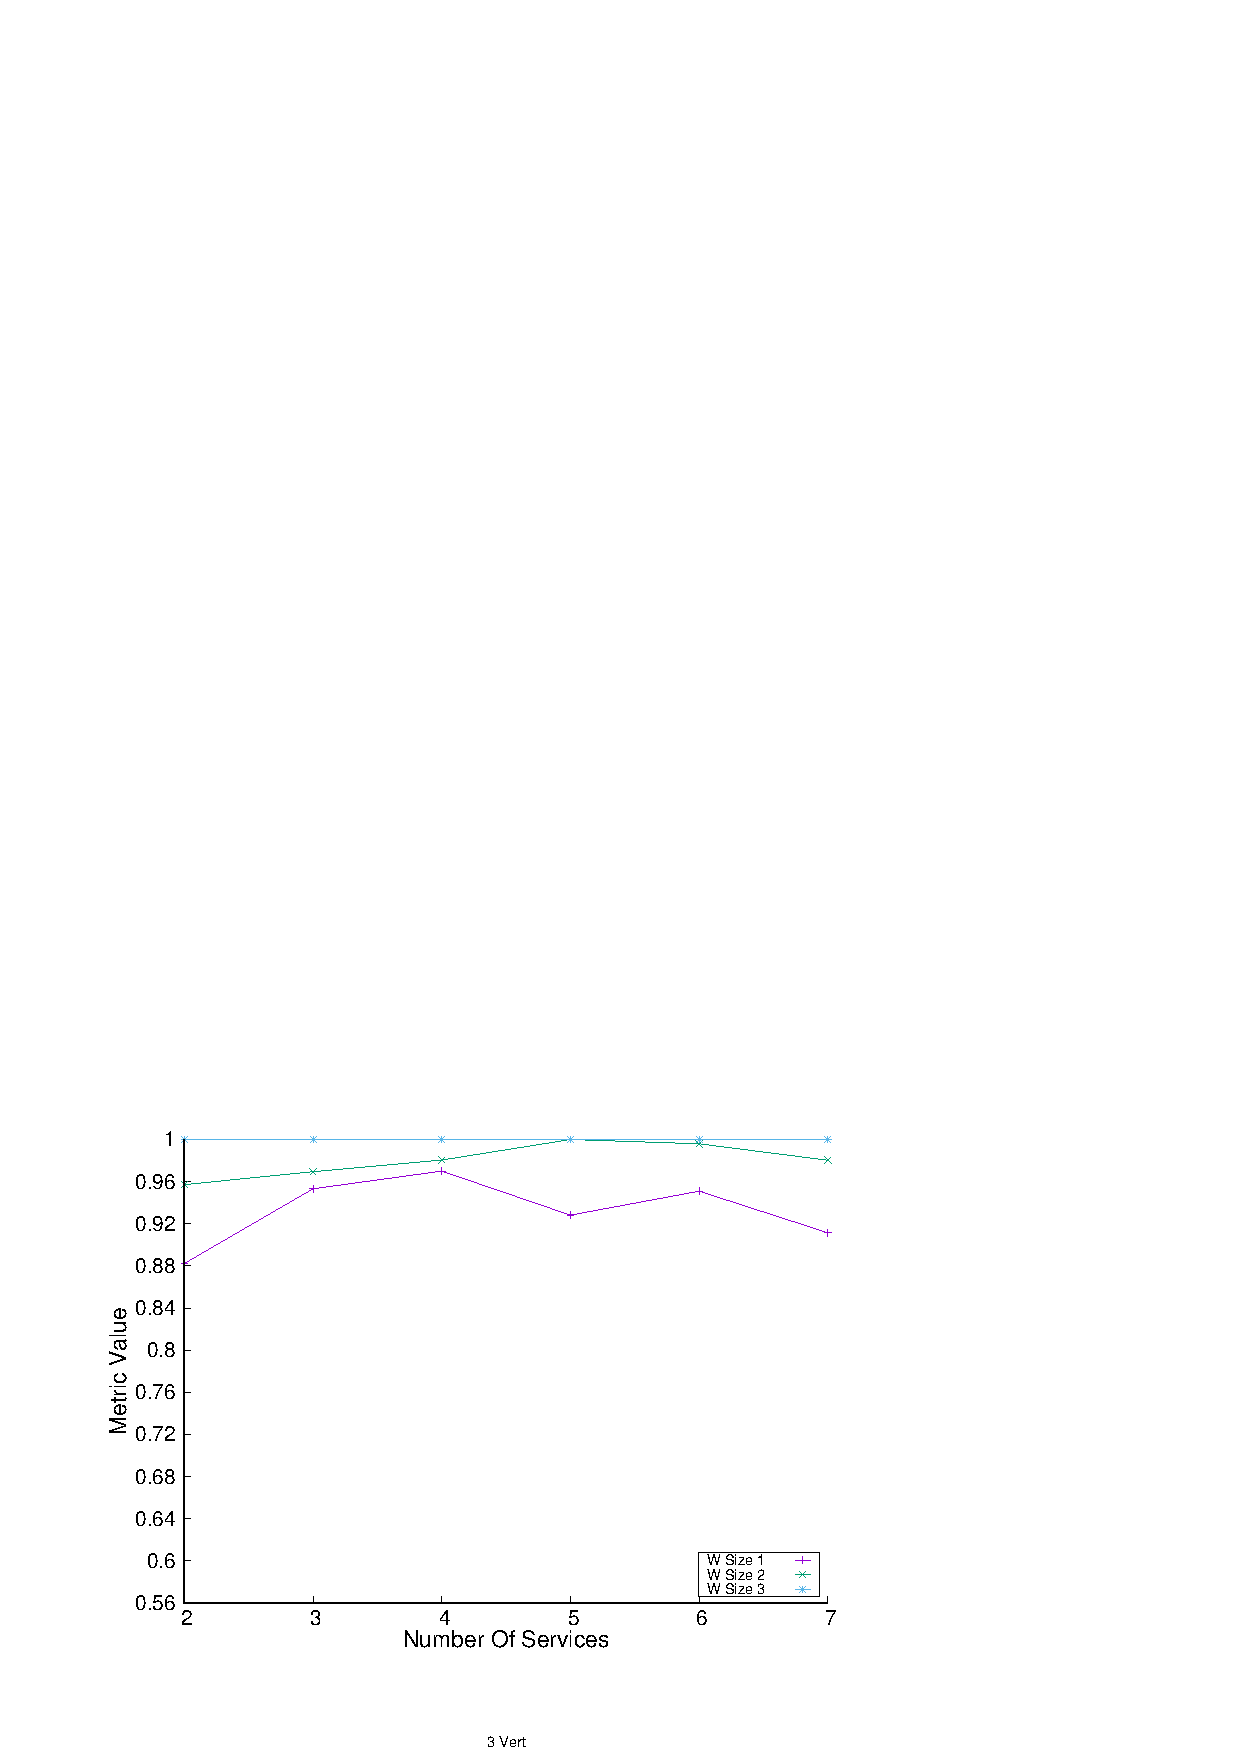
\includegraphics[width=\textwidth]{Images/graphs/window_quality_performance_diff_perce_n7_s7_20_100_n3}
    \caption{3 vertices}
    \label{fig:quality_window_perce_wide_3n}
  \end{subfigure}
  \hfill
  \begin{subfigure}{0.33\textwidth}
    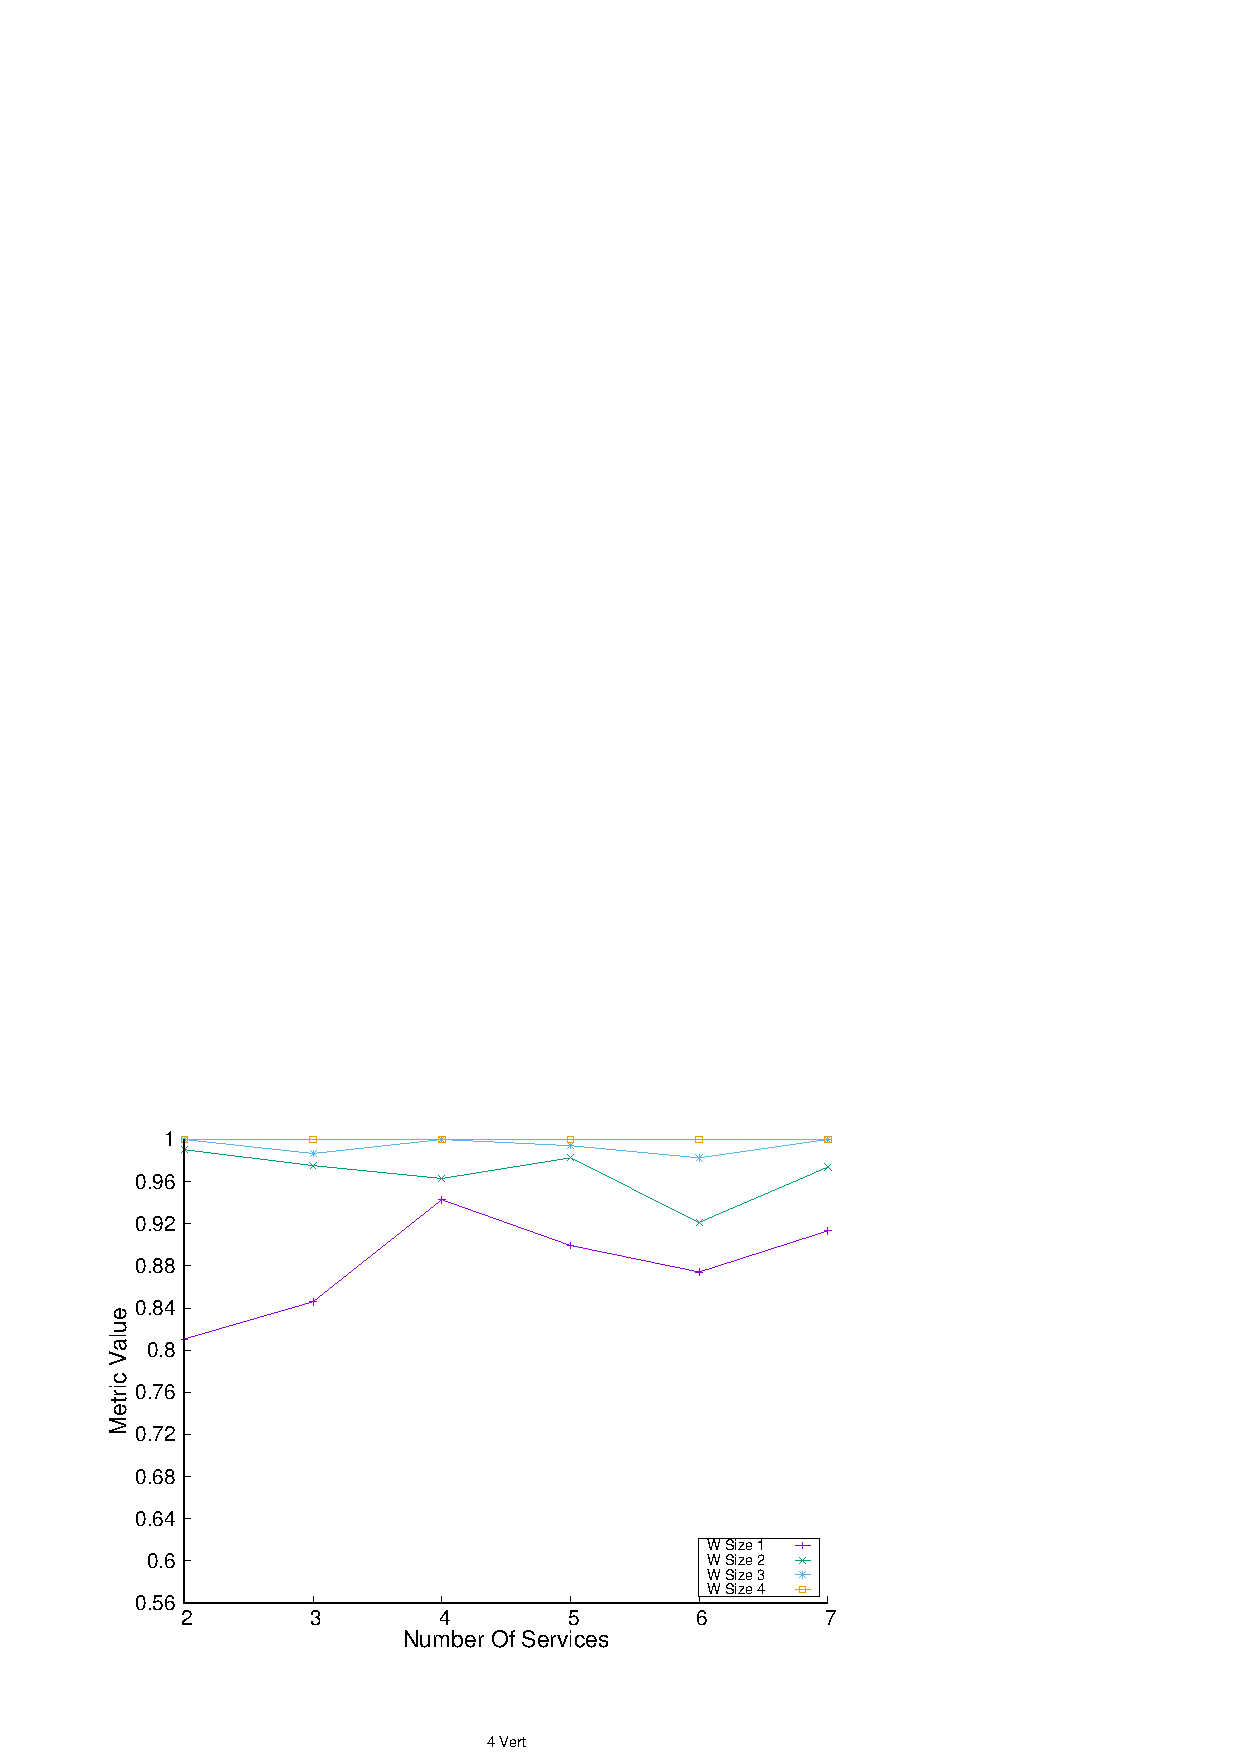
\includegraphics[width=\textwidth]{Images/graphs/window_quality_performance_diff_perce_n7_s7_20_100_n4}
    \caption{4 vertices}
    \label{fig:quality_window_perce_wide_4n}
  \end{subfigure}
  \hfill
  \begin{subfigure}{0.33\textwidth}
    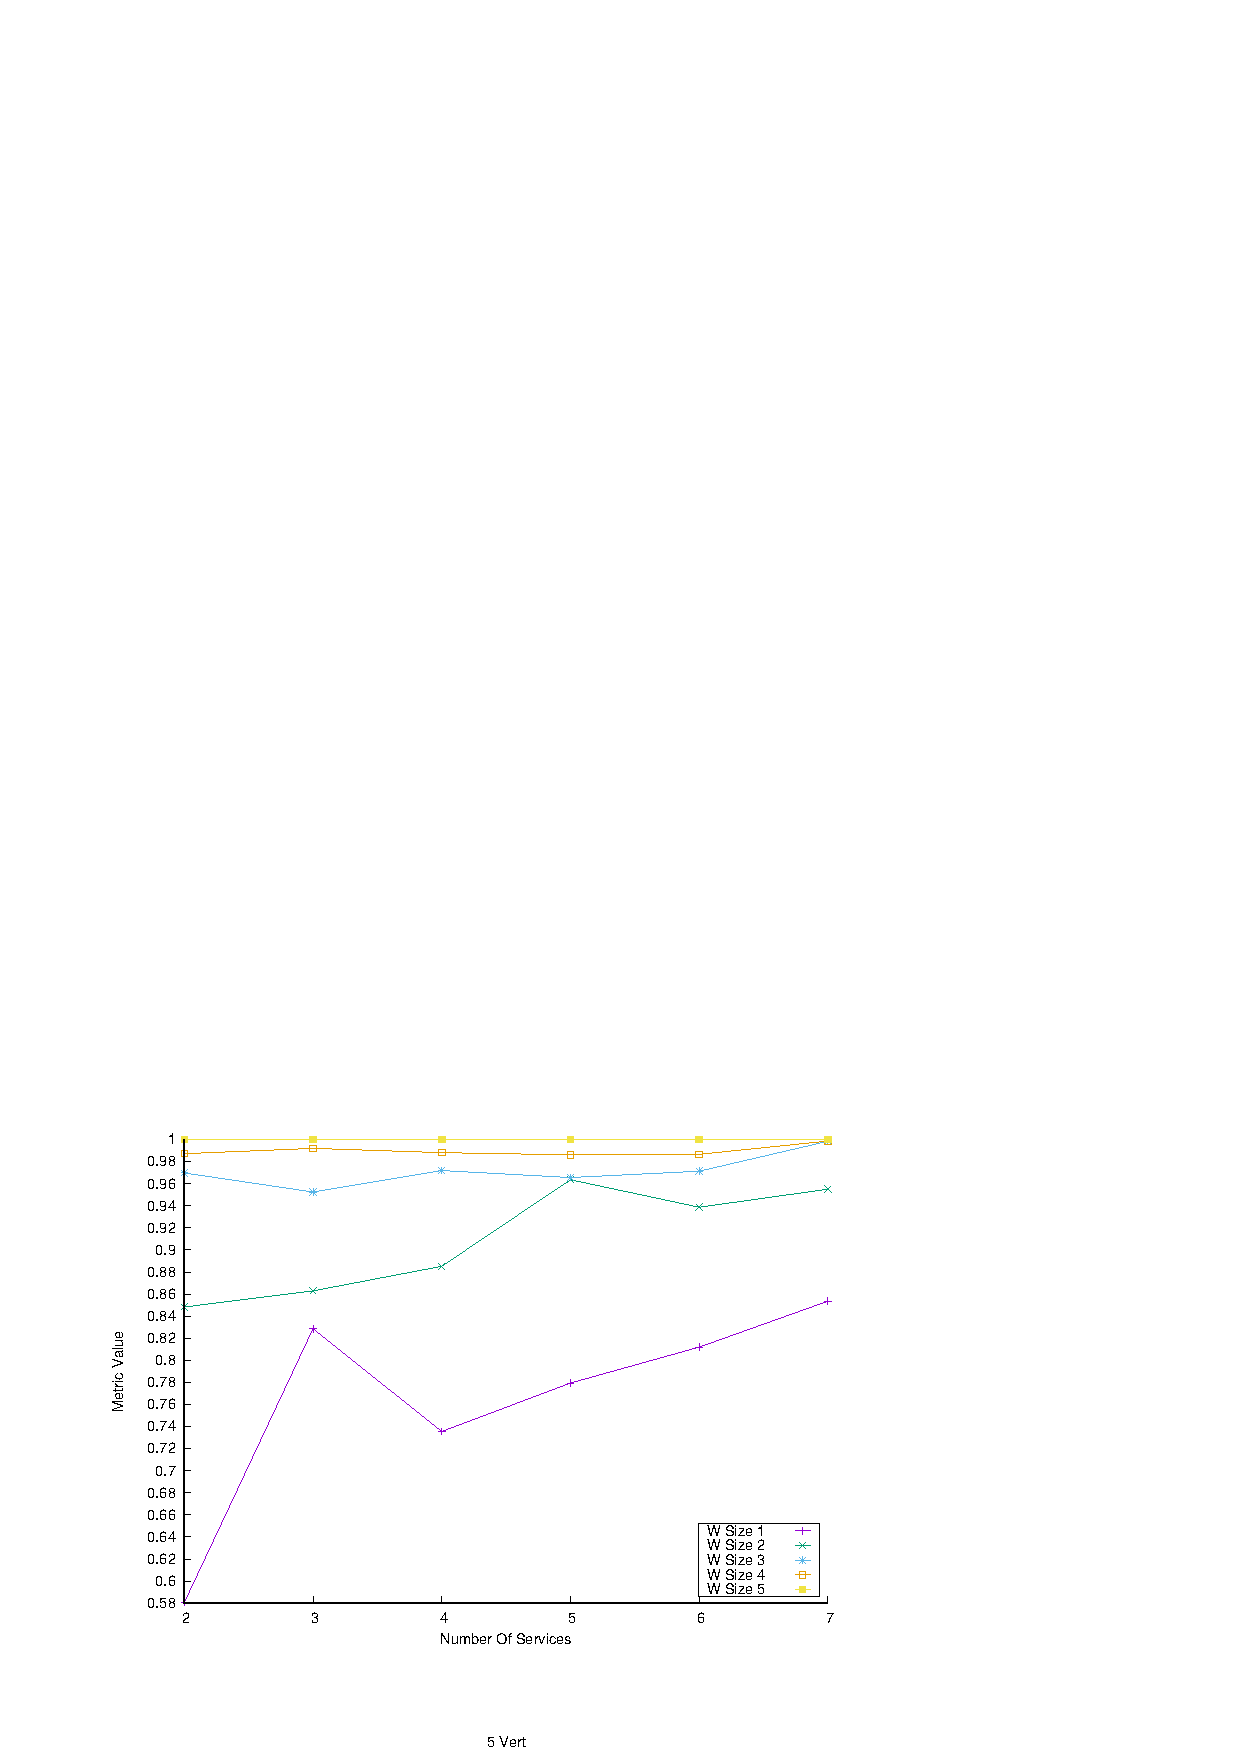
\includegraphics[width=\textwidth]{Images/graphs/window_quality_performance_diff_perce_n7_s7_20_100_n5}
    \caption{5 vertices}
    \label{fig:quality_window_perce_wide_5n}
  \end{subfigure}
  \hfill
  \begin{subfigure}{0.33\textwidth}
    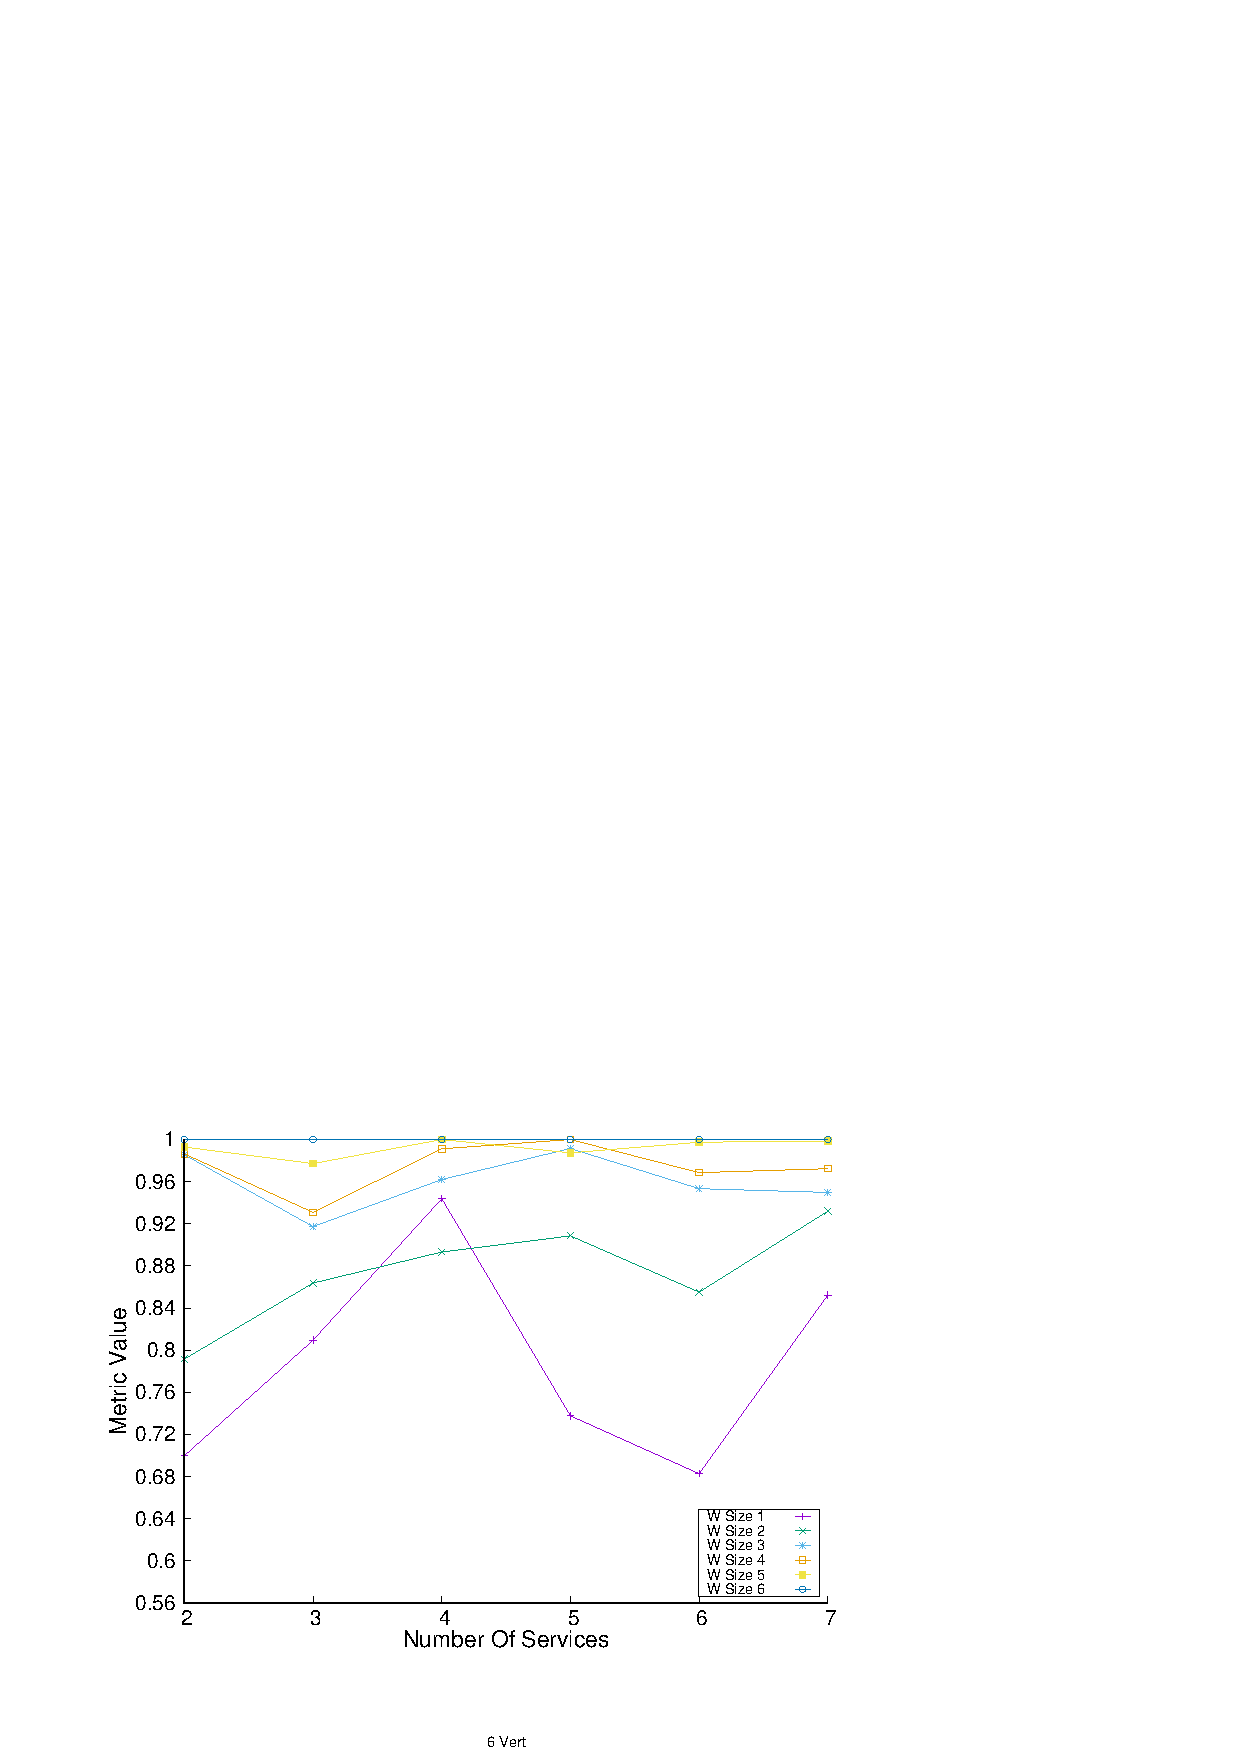
\includegraphics[width=\textwidth]{Images/graphs/window_quality_performance_diff_perce_n7_s7_20_100_n6}
    \caption{6 vertices}
    \label{fig:quality_window_perce_wide_6n}
  \end{subfigure}
  \begin{subfigure}{0.33\textwidth}
    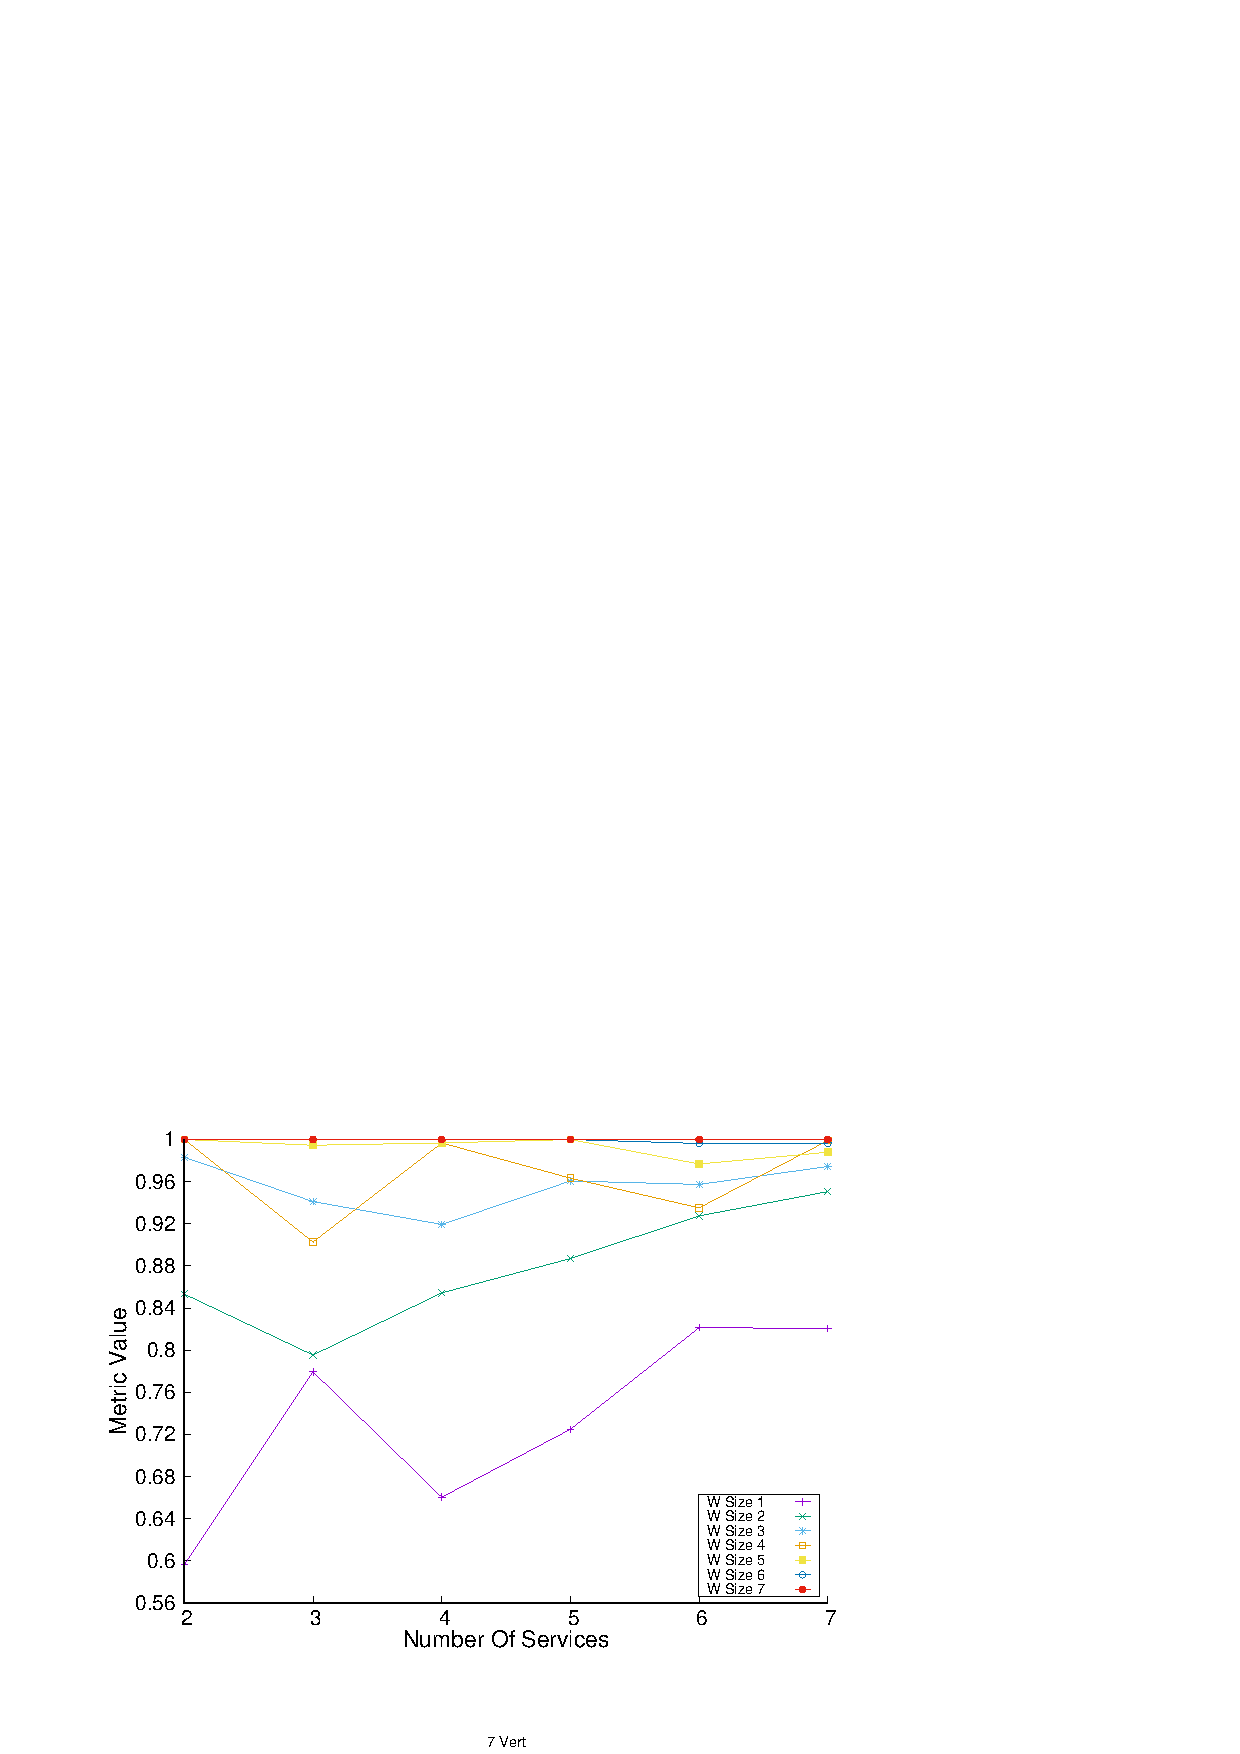
\includegraphics[width=\textwidth]{Images/graphs/window_quality_performance_diff_perce_n7_s7_20_100_n7}
    \caption{7 vertices}
    \label{fig:quality_window_perce_wide_7n}
  \end{subfigure}
  % \hfill
  % \begin{subfigure}{0.33\textwidth}
  %   \includegraphics[width=\textwidth]{Images/graphs/quality_plot_average_n7.eps}
  %   \caption{7 vertices}
  %   \label{fig:third}
  % \end{subfigure}
  \caption{Evaluation of Quality Using the \emph{Quantitative} Metric in a \wide Profile Configuration.}  \label{fig:quality_window_perce_wide}
\end{figure*}


\begin{figure*}[!htb]
  \centering
  \begin{subfigure}{0.33\textwidth}
    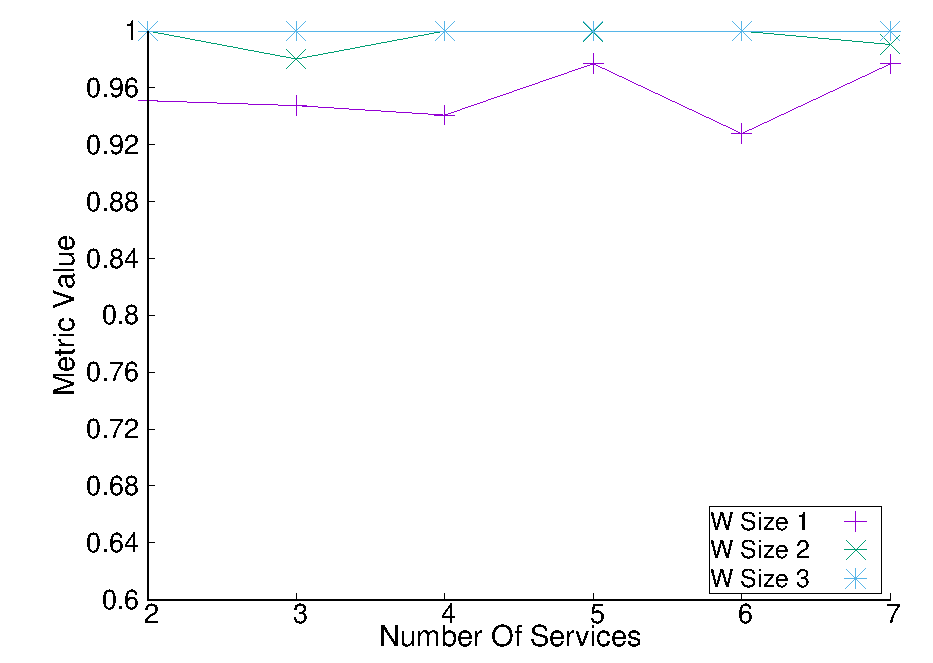
\includegraphics[width=\textwidth]{Images/graphs/window_quality_performance_diff_perce_n7_s7_50_89_n3}
    \caption{3 vertices}
    \label{fig:quality_window_average_perce_3n}
  \end{subfigure}
  \hfill
  \begin{subfigure}{0.33\textwidth}
    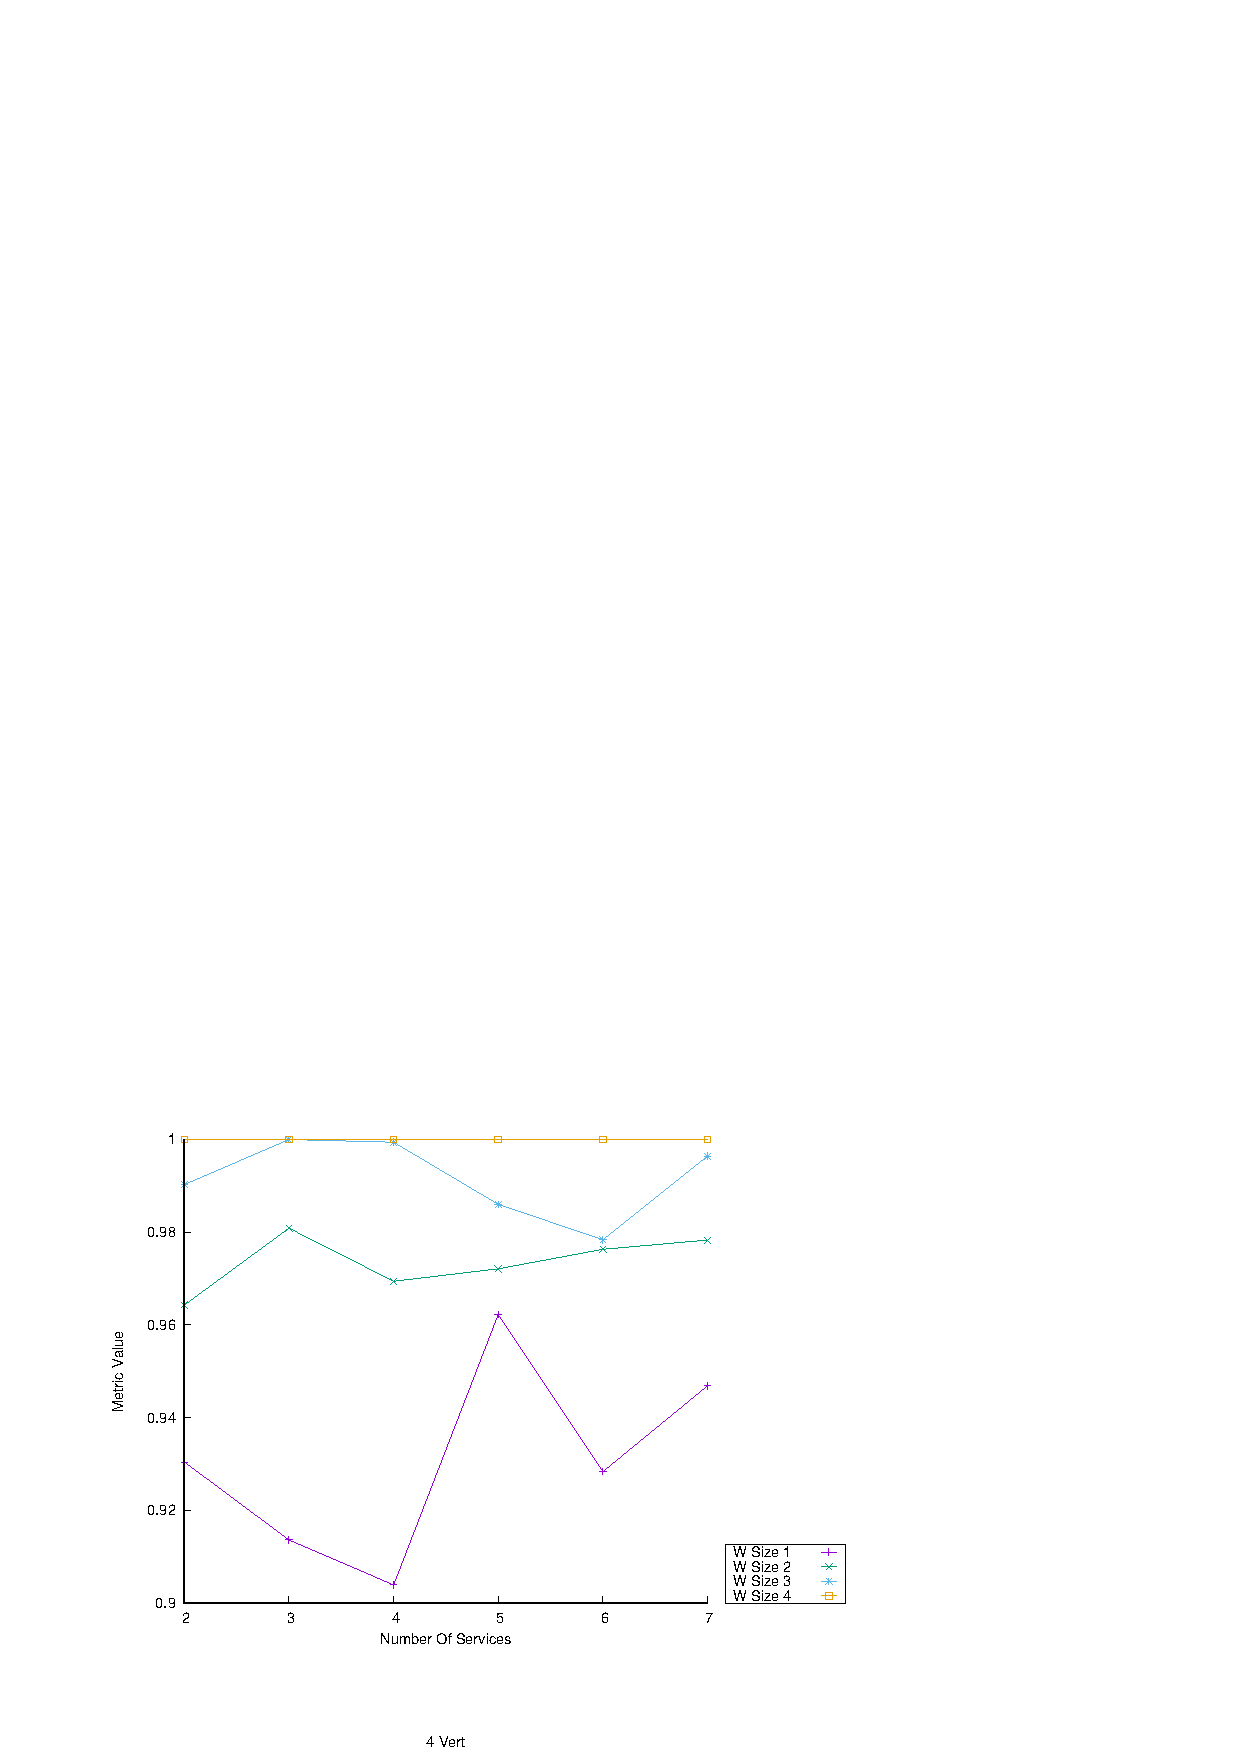
\includegraphics[width=\textwidth]{Images/graphs/window_quality_performance_diff_perce_n7_s7_50_89_n4}
    \caption{4 vertices}
    \label{fig:quality_window_average_perce_4n}

  \end{subfigure}
  \hfill
  \begin{subfigure}{0.33\textwidth}
    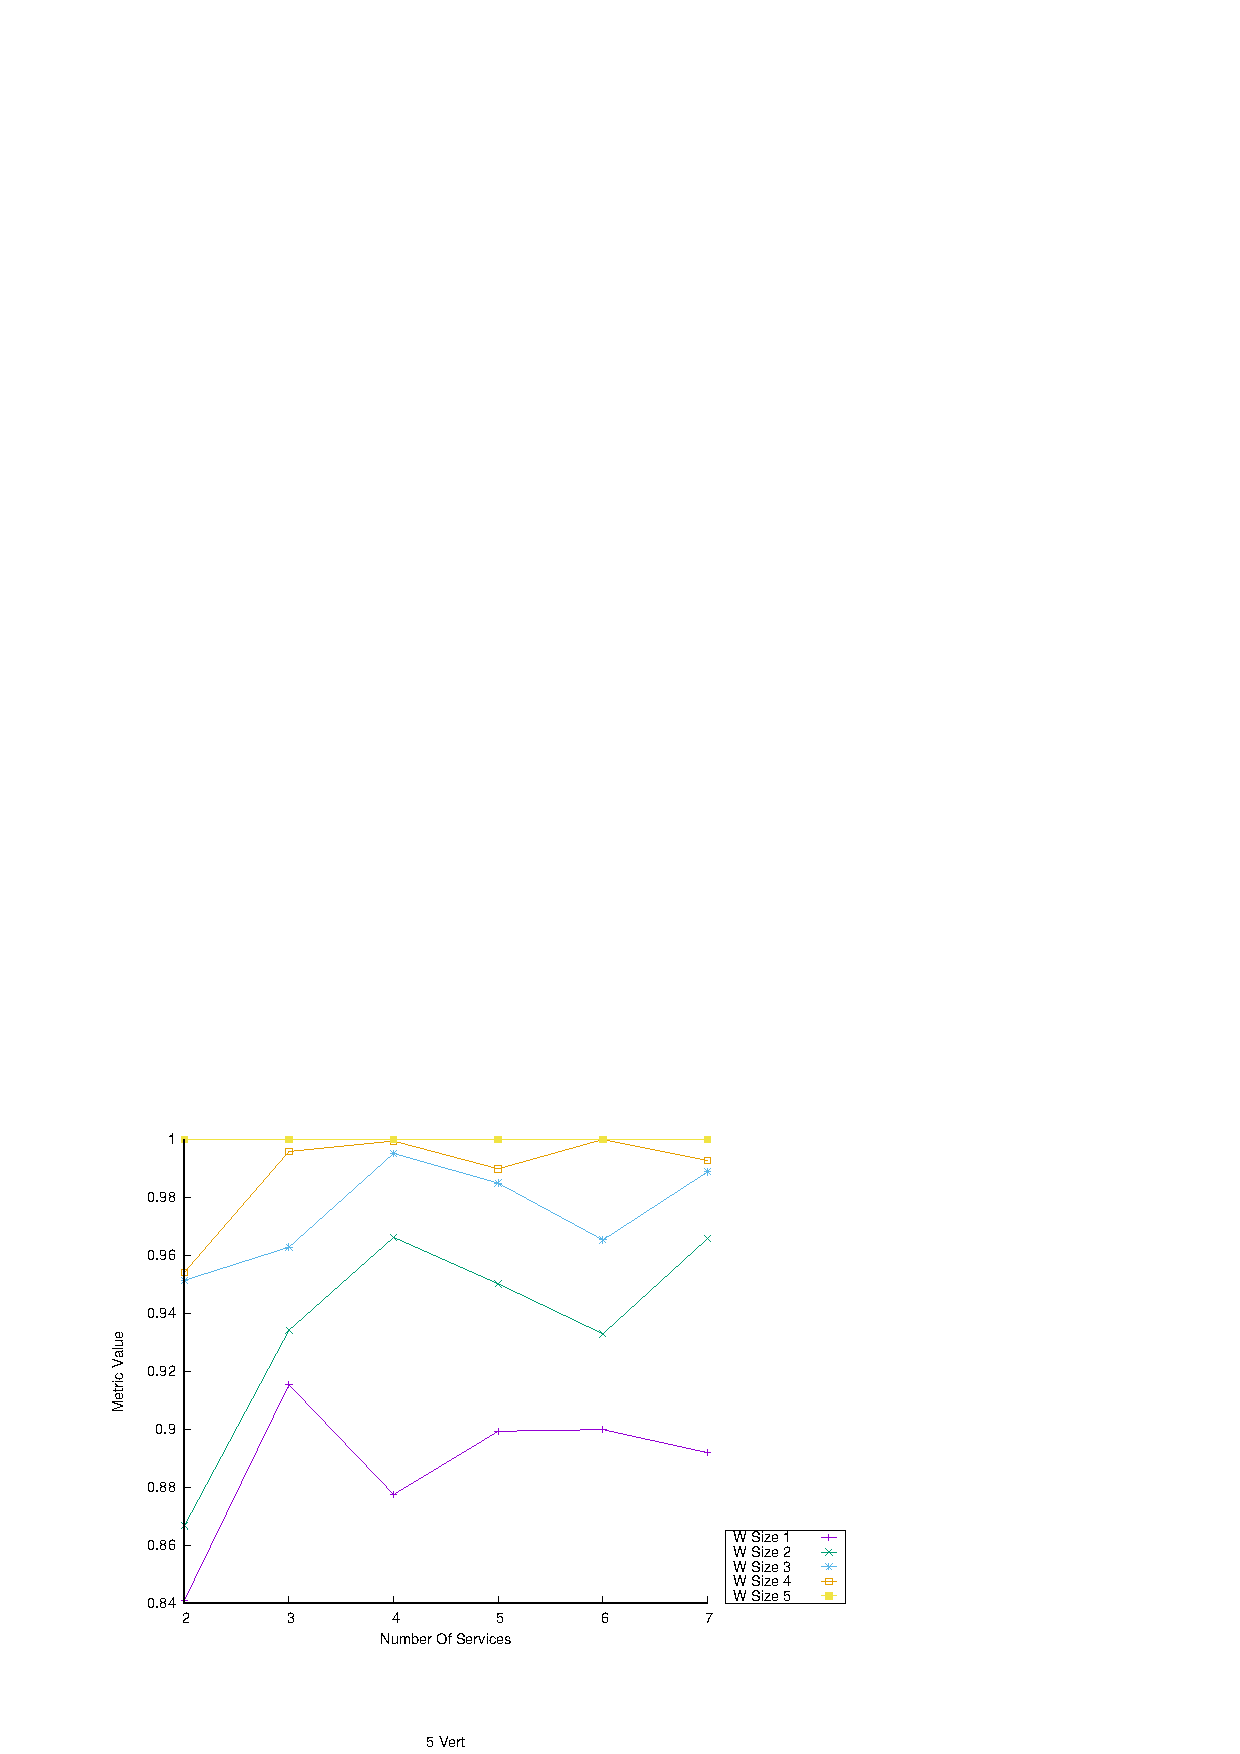
\includegraphics[width=\textwidth]{Images/graphs/window_quality_performance_diff_perce_n7_s7_50_89_n5}
    \caption{5 vertices}
    \label{fig:quality_window_average_perce_5n}
  \end{subfigure}
  \hfill
  \begin{subfigure}{0.33\textwidth}
    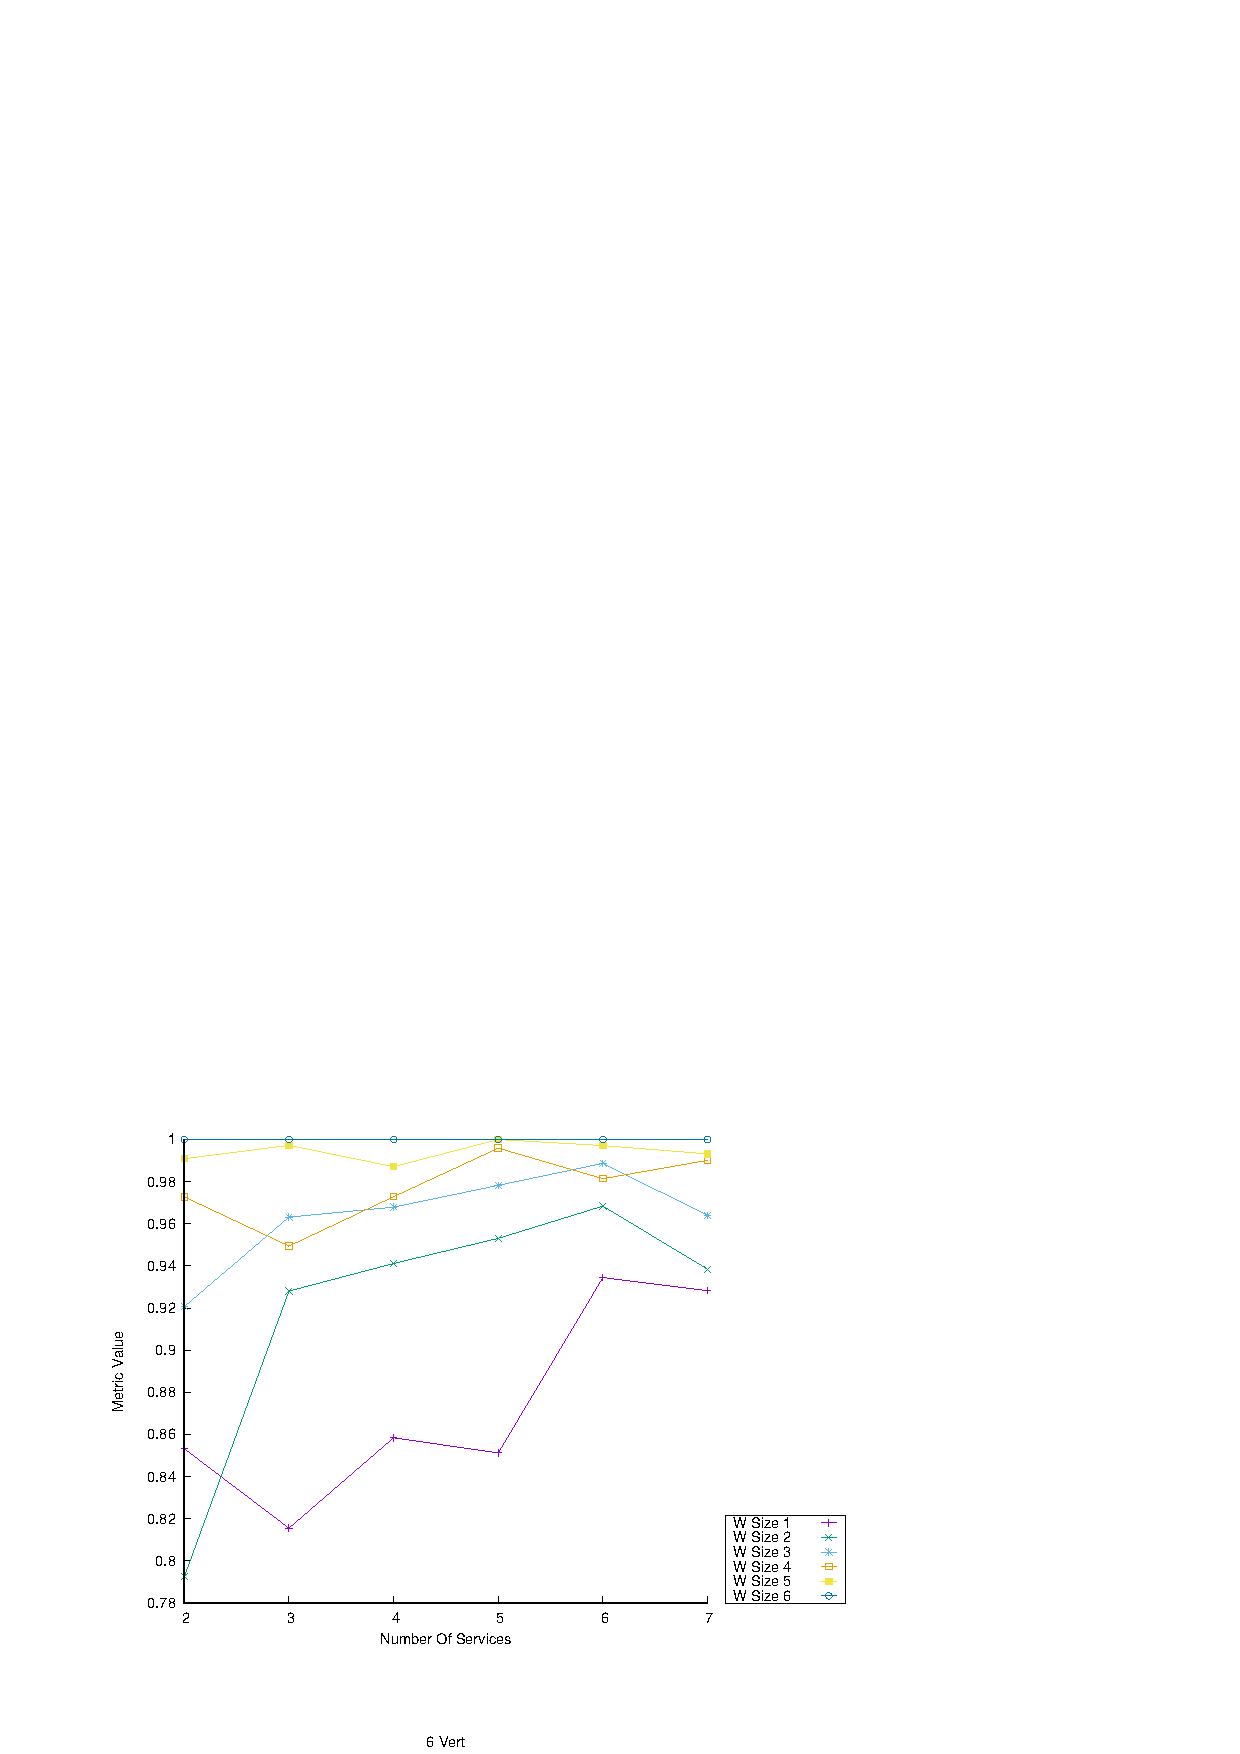
\includegraphics[width=\textwidth]{Images/graphs/window_quality_performance_diff_perce_n7_s7_50_89_n6}
    \caption{6 vertices}
    \label{fig:quality_window_average_perce_6n}
  \end{subfigure}
  \begin{subfigure}{0.33\textwidth}
    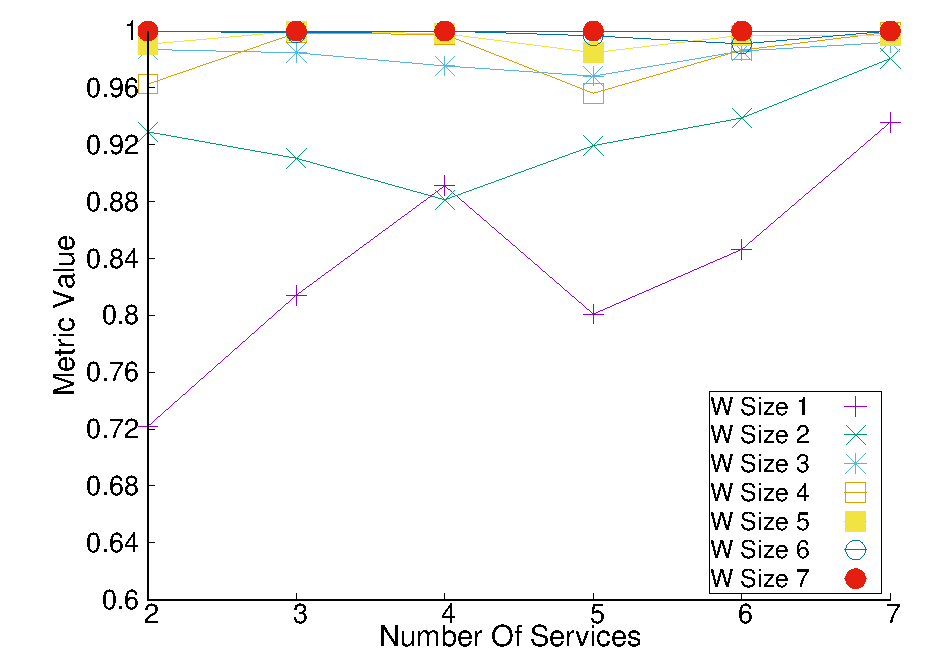
\includegraphics[width=\textwidth]{Images/graphs/window_quality_performance_diff_perce_n7_s7_50_89_n7}
    \caption{7 vertices}
    \label{fig:quality_window_average_perce_7n}
  \end{subfigure}
  % \hfill
  % \begin{subfigure}{0.33\textwidth}
  %   \includegraphics[width=\textwidth]{Images/graphs/quality_plot_average_n7.eps}
  %   \caption{7 vertices}
  %   \label{fig:third}
  % \end{subfigure}
  \caption{Evaluation of Quality Using the \emph{Quantitative} Metric in a \average Profile Configuration.}  \label{fig:quality_window_average_perce}
\end{figure*}


\begin{figure*}[!htb]
  \centering
  \begin{subfigure}{0.33\textwidth}
    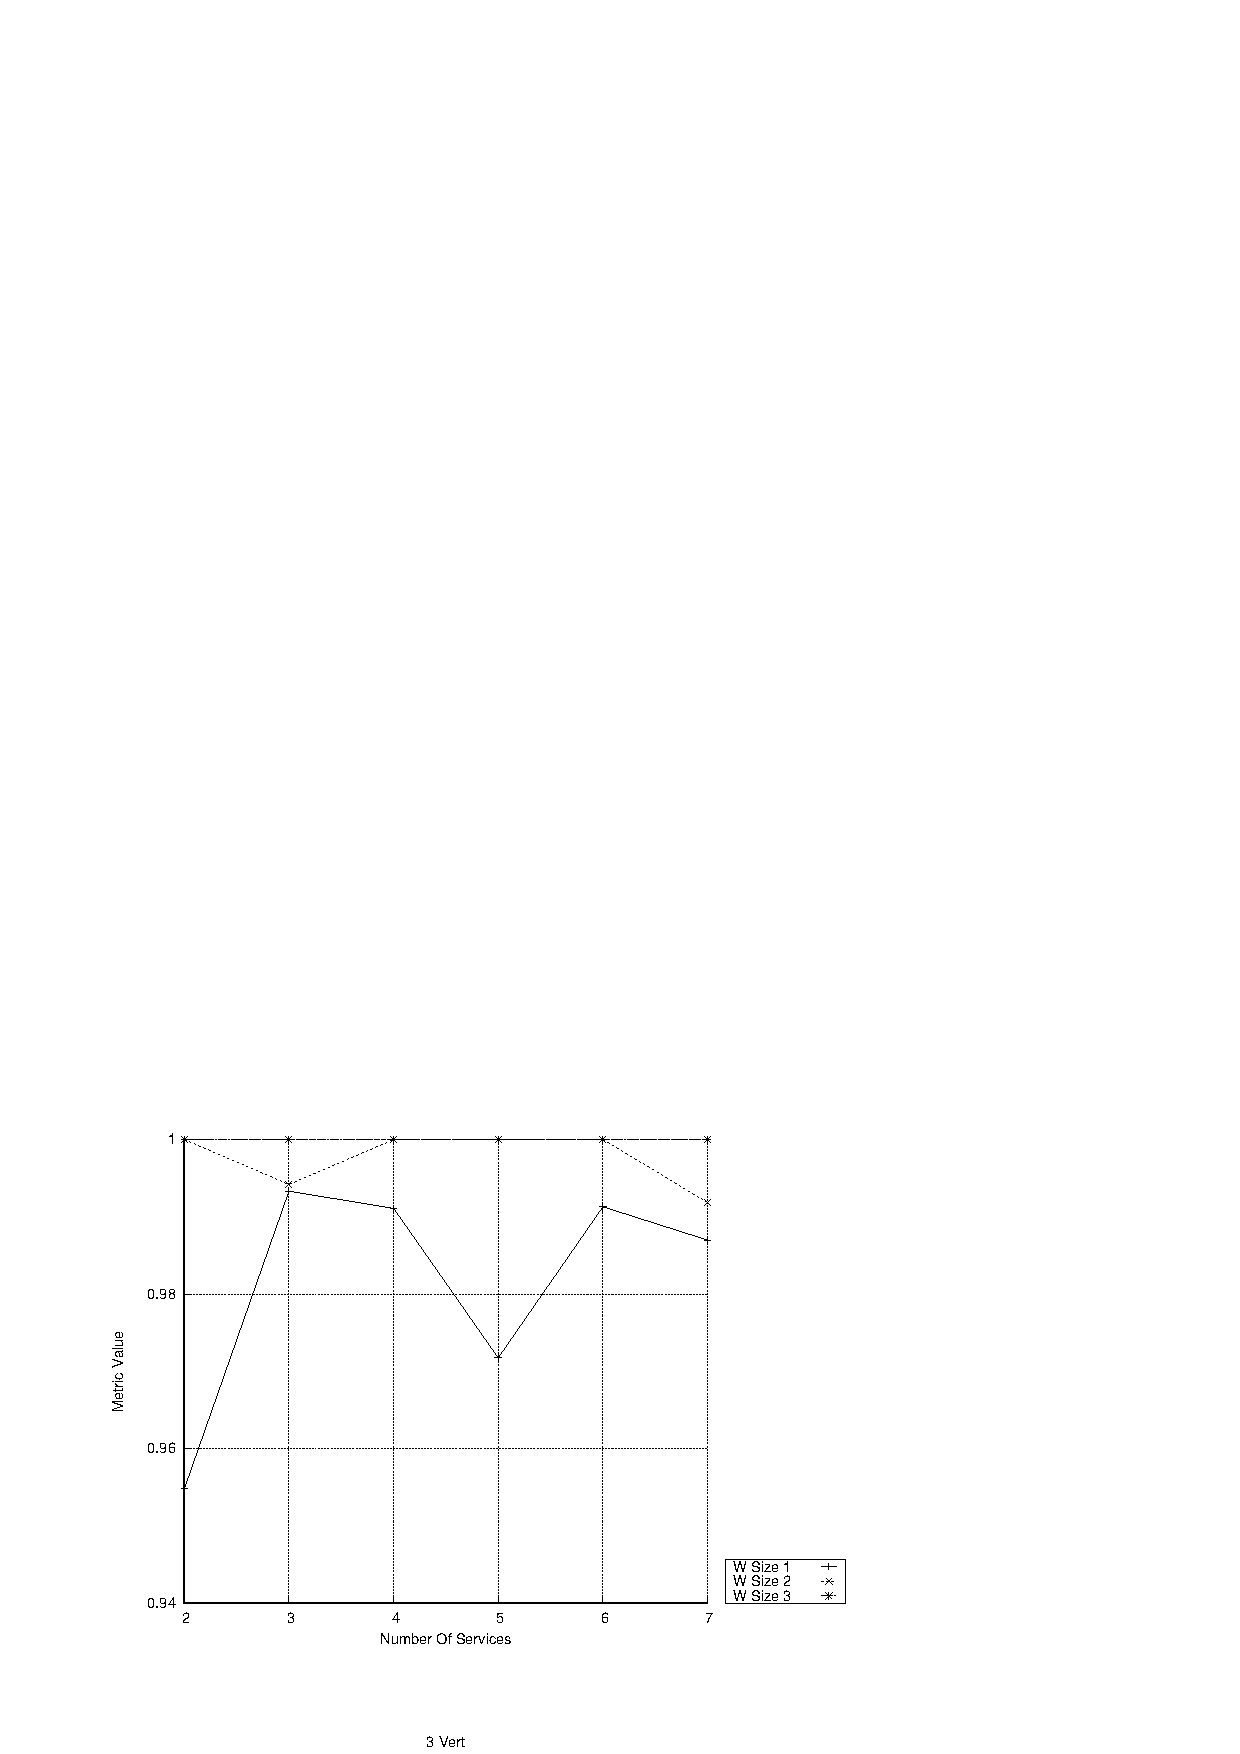
\includegraphics[width=\textwidth]{Images/graphs/window_quality_performance_diff_qual_n7_s7_20_100_n3}
    \caption{3 vertices}
    \label{fig:quality_window_wide_qualitative_n3}
  \end{subfigure}
  \hfill
  \begin{subfigure}{0.33\textwidth}
    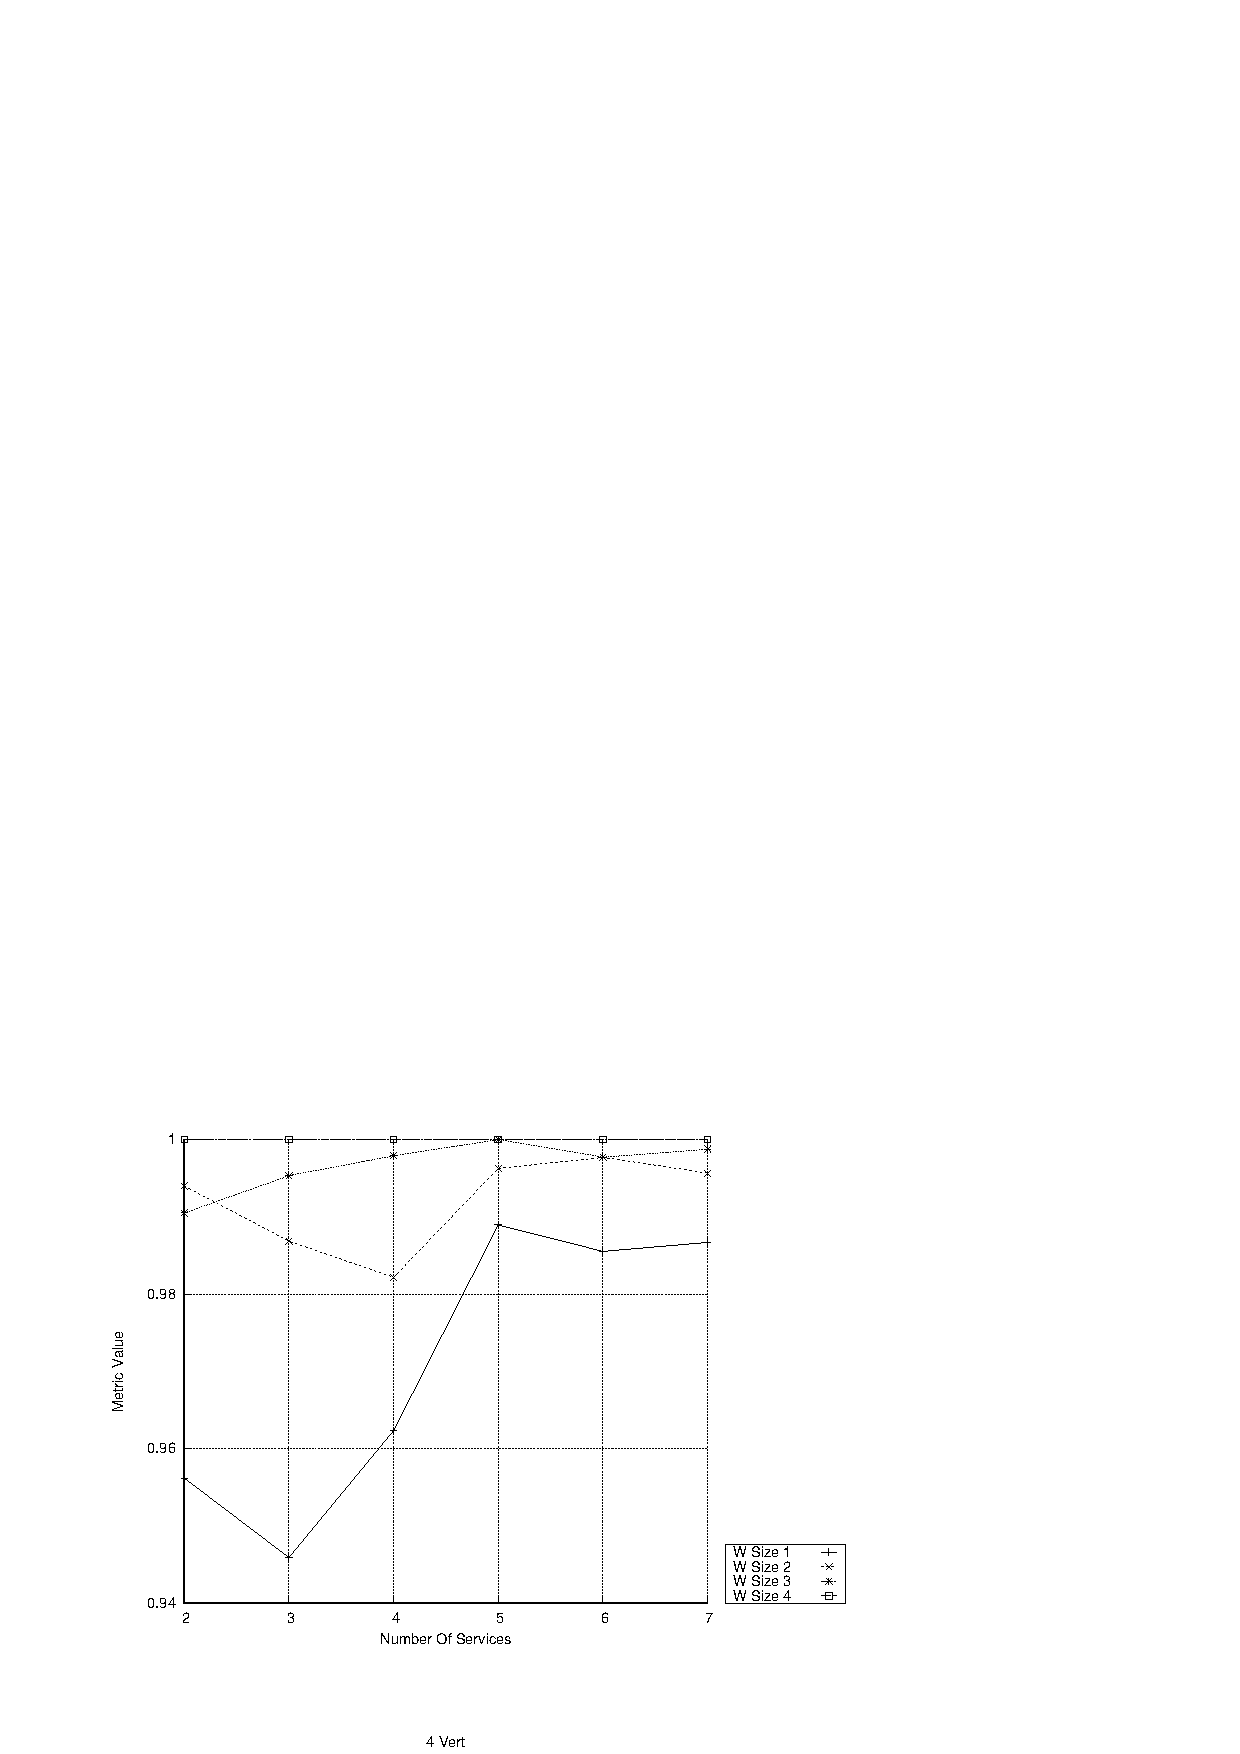
\includegraphics[width=\textwidth]{Images/graphs/window_quality_performance_diff_qual_n7_s7_20_100_n4}
    \caption{4 vertices}
    \label{fig:quality_window_wide_qualitative_n4}
  \end{subfigure}
  \hfill
  \begin{subfigure}{0.33\textwidth}
    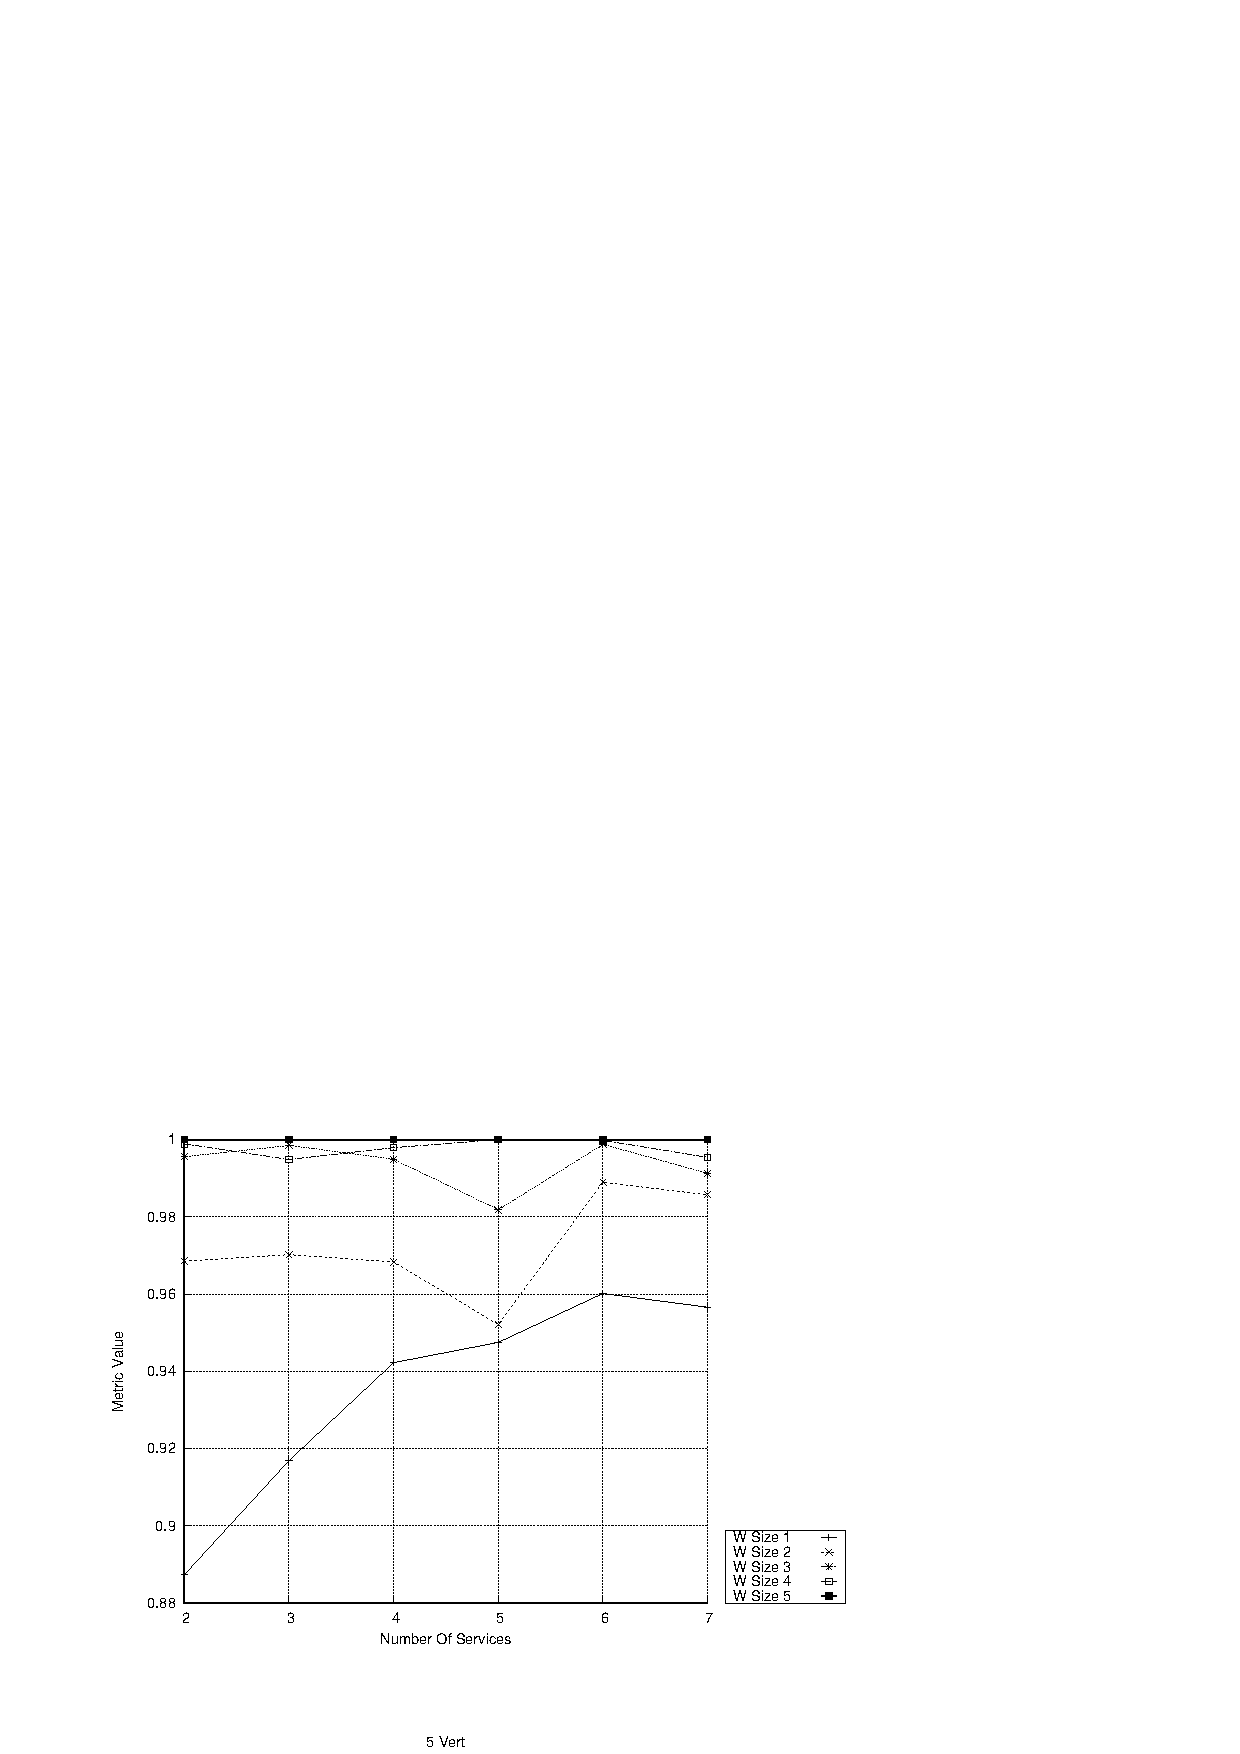
\includegraphics[width=\textwidth]{Images/graphs/window_quality_performance_diff_qual_n7_s7_20_100_n5}
    \caption{5 vertices}
    \label{fig:quality_window_average_qualitative_n5}
  \end{subfigure}
  \hfill
  \begin{subfigure}{0.33\textwidth}
    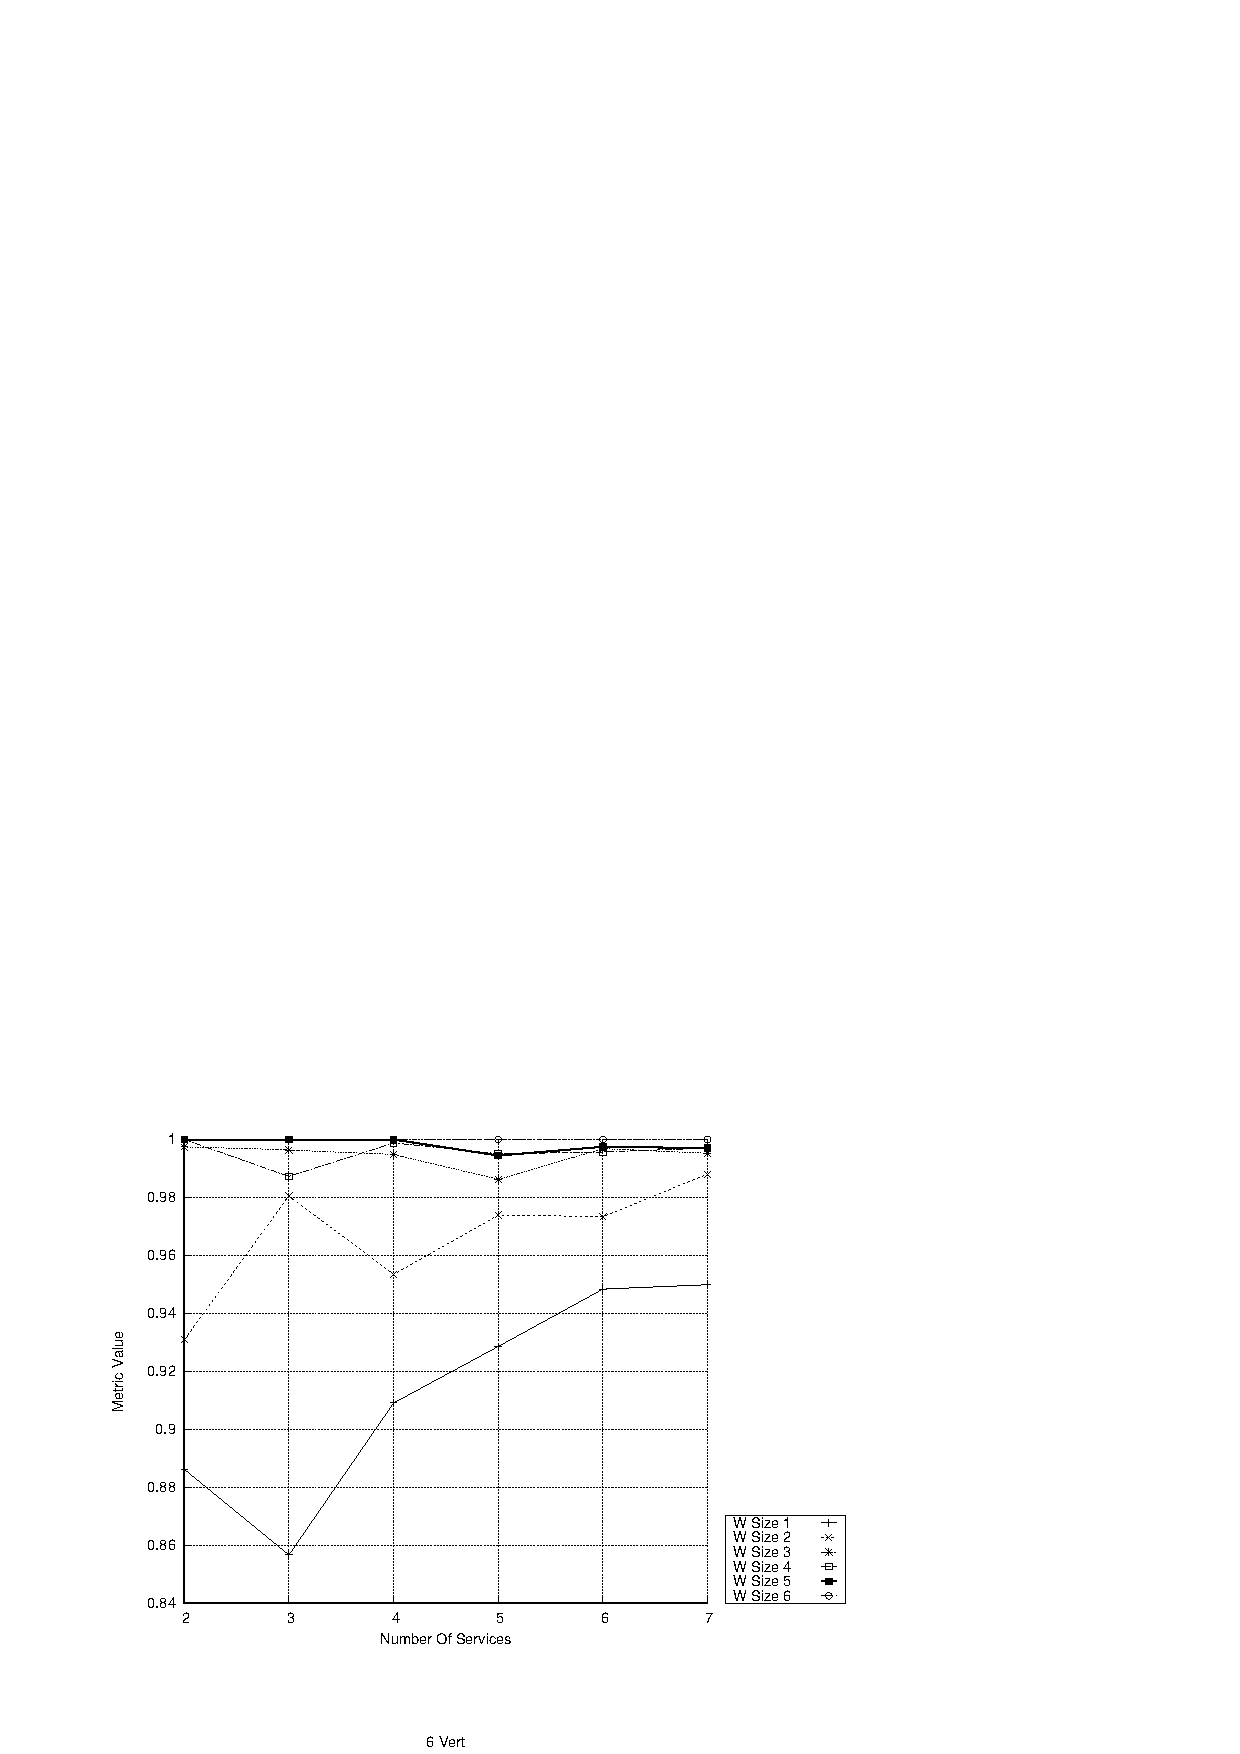
\includegraphics[width=\textwidth]{Images/graphs/window_quality_performance_diff_qual_n7_s7_20_100_n6}
    \caption{6 vertices}
    \label{fig:quality_window_wide_qualitative_n6}
  \end{subfigure}
  \begin{subfigure}{0.33\textwidth}
    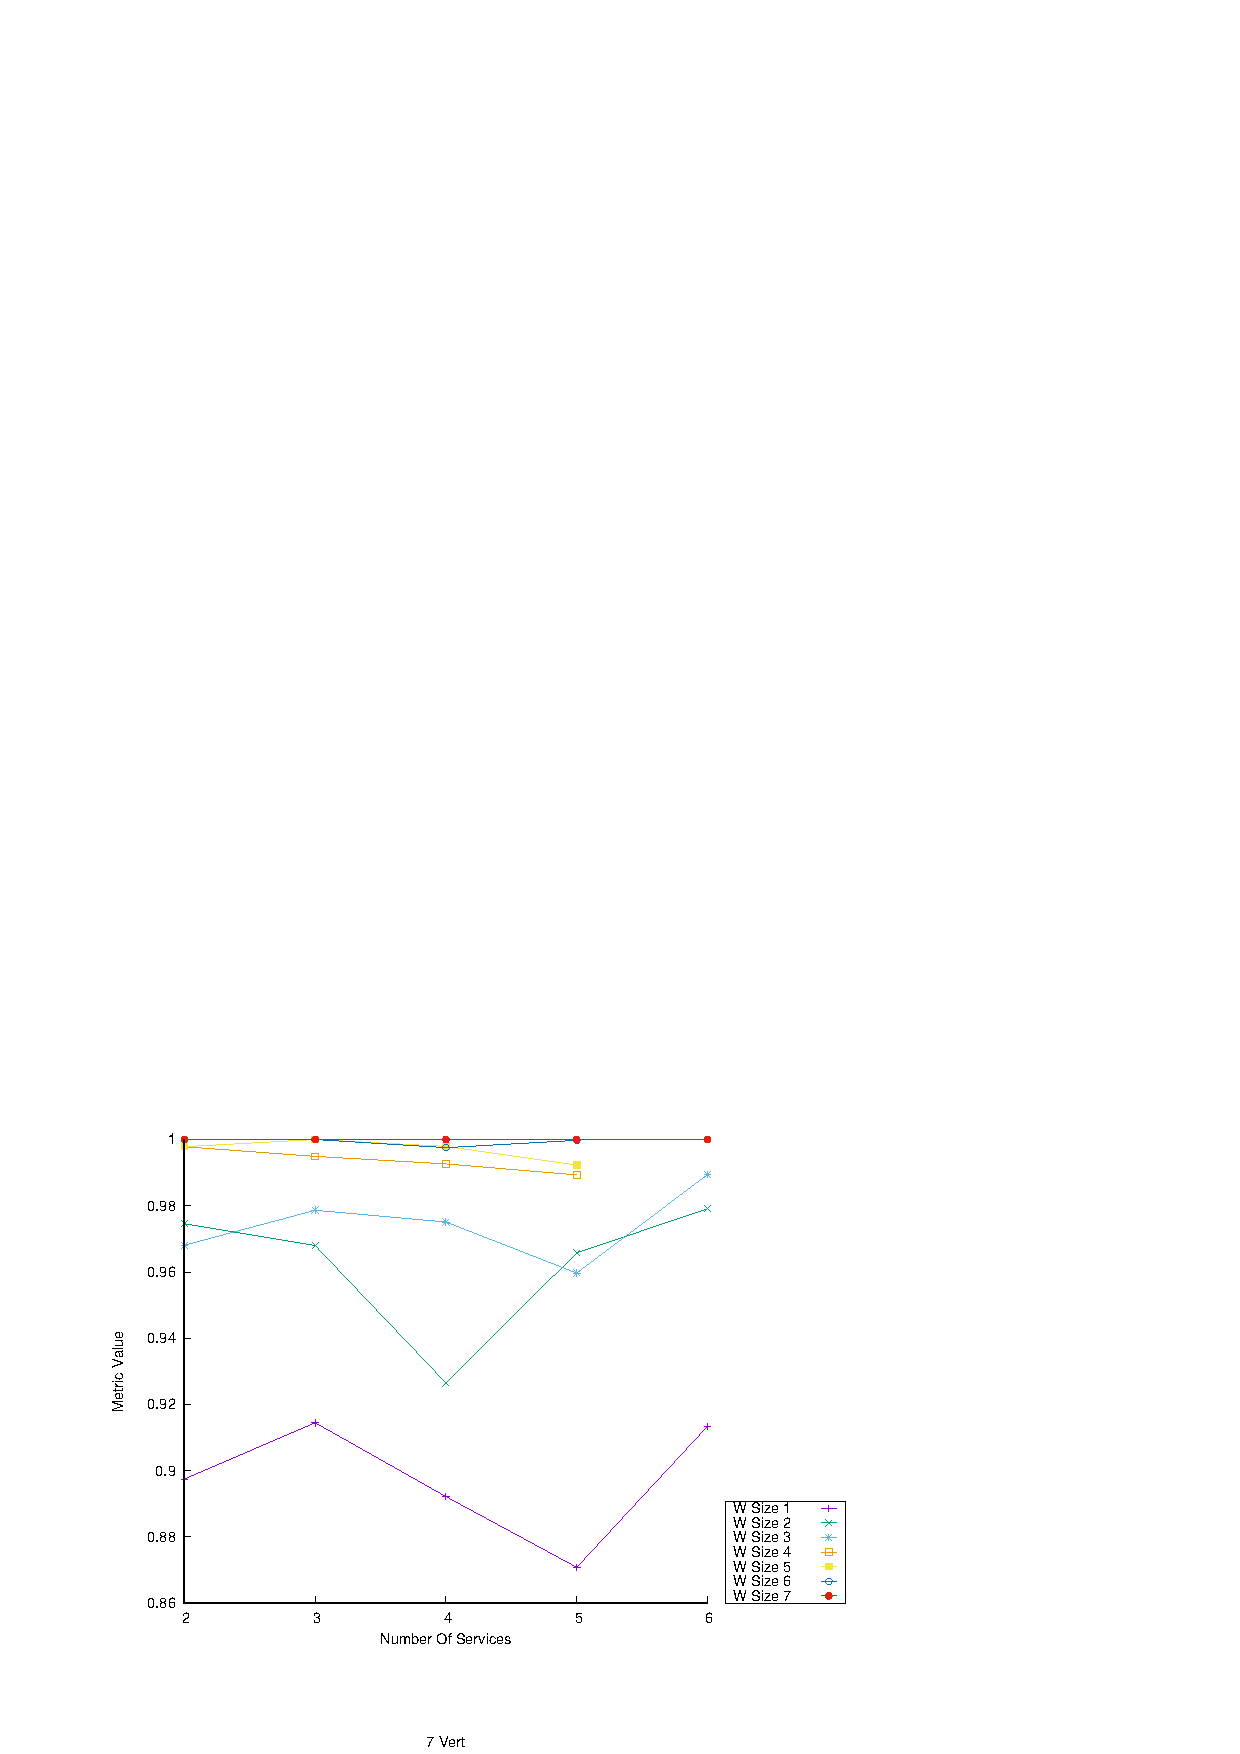
\includegraphics[width=\textwidth]{Images/graphs/window_quality_performance_diff_qual_n7_s7_20_100_n7}
    \caption{7 vertices}
    \label{fig:quality_window_wide_qualitative_n7}
  \end{subfigure}

  \caption{Evaluation of Quality Using the \emph{Qualitative} Metric in a \wide Profile Configuration.}  \label{fig:quality_window_wide_qualitative}
\end{figure*}

\begin{figure*}[!htb]
  \centering
  \begin{subfigure}{0.33\textwidth}
    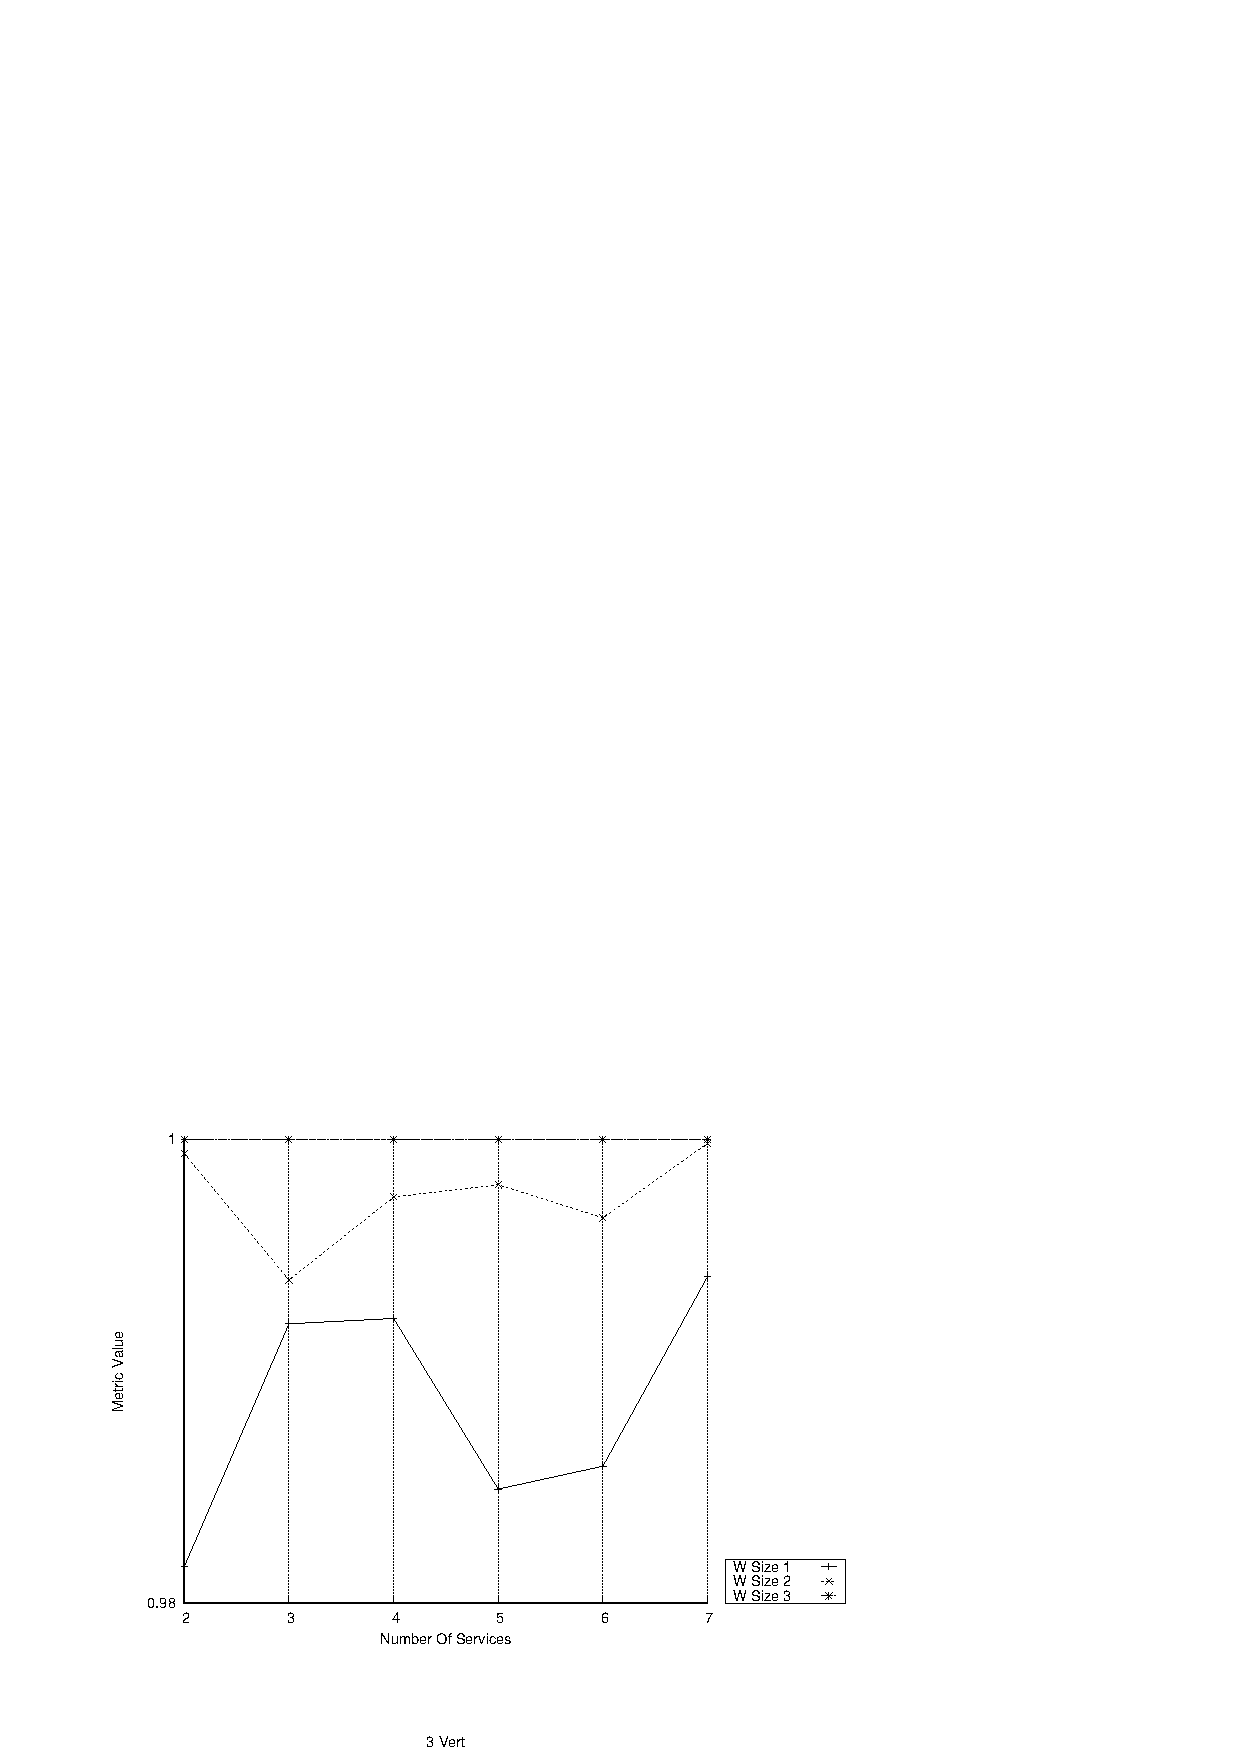
\includegraphics[width=\textwidth]{Images/graphs/window_quality_performance_diff_qual_n7_s7_50_80_n3}
    \caption{3 vertices}
    \label{fig:quality_window_average_qualitative_n3}
  \end{subfigure}
  \hfill
  \begin{subfigure}{0.33\textwidth}
    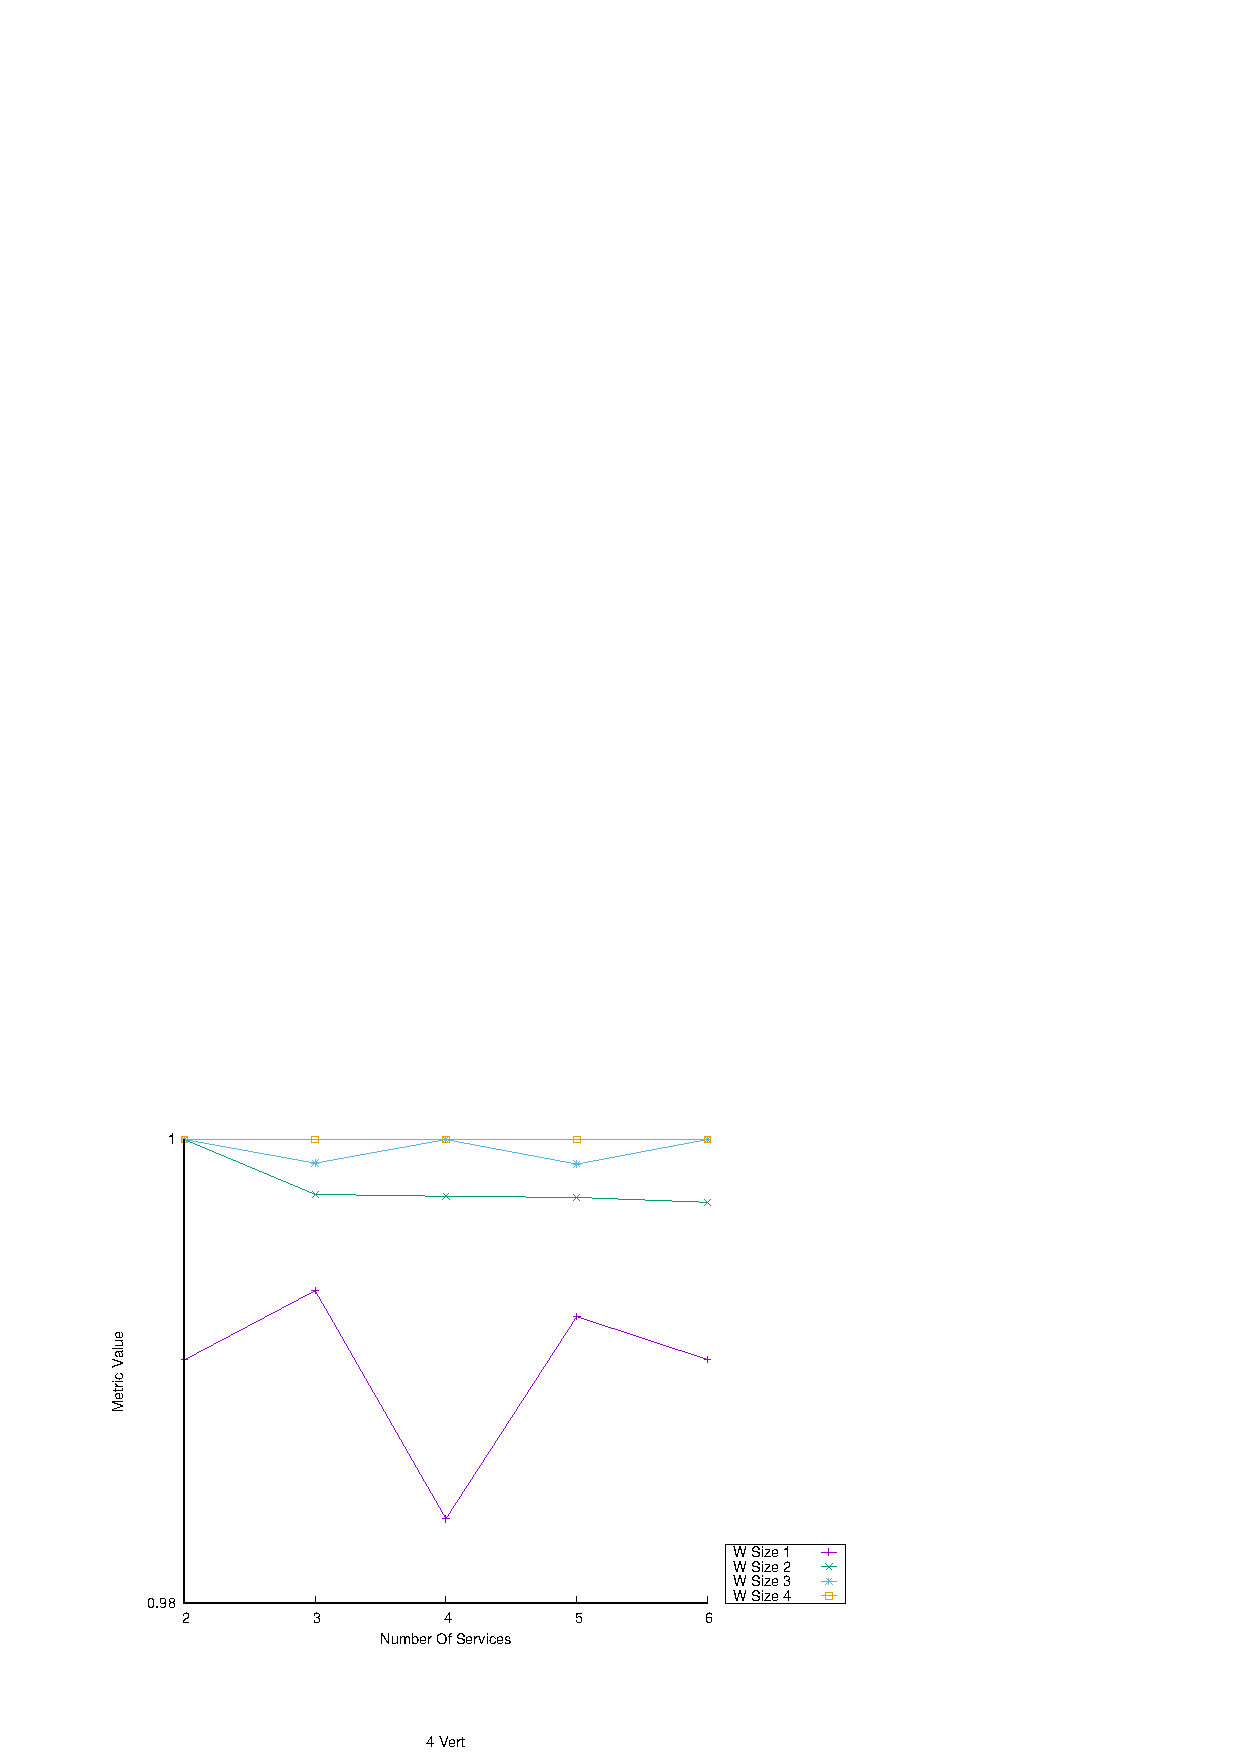
\includegraphics[width=\textwidth]{Images/graphs/window_quality_performance_diff_qual_n7_s7_50_80_n4}
    \caption{4 vertices}
    \label{fig:quality_window_average_qualitative_n4}
  \end{subfigure}
  \hfill
  \begin{subfigure}{0.33\textwidth}
    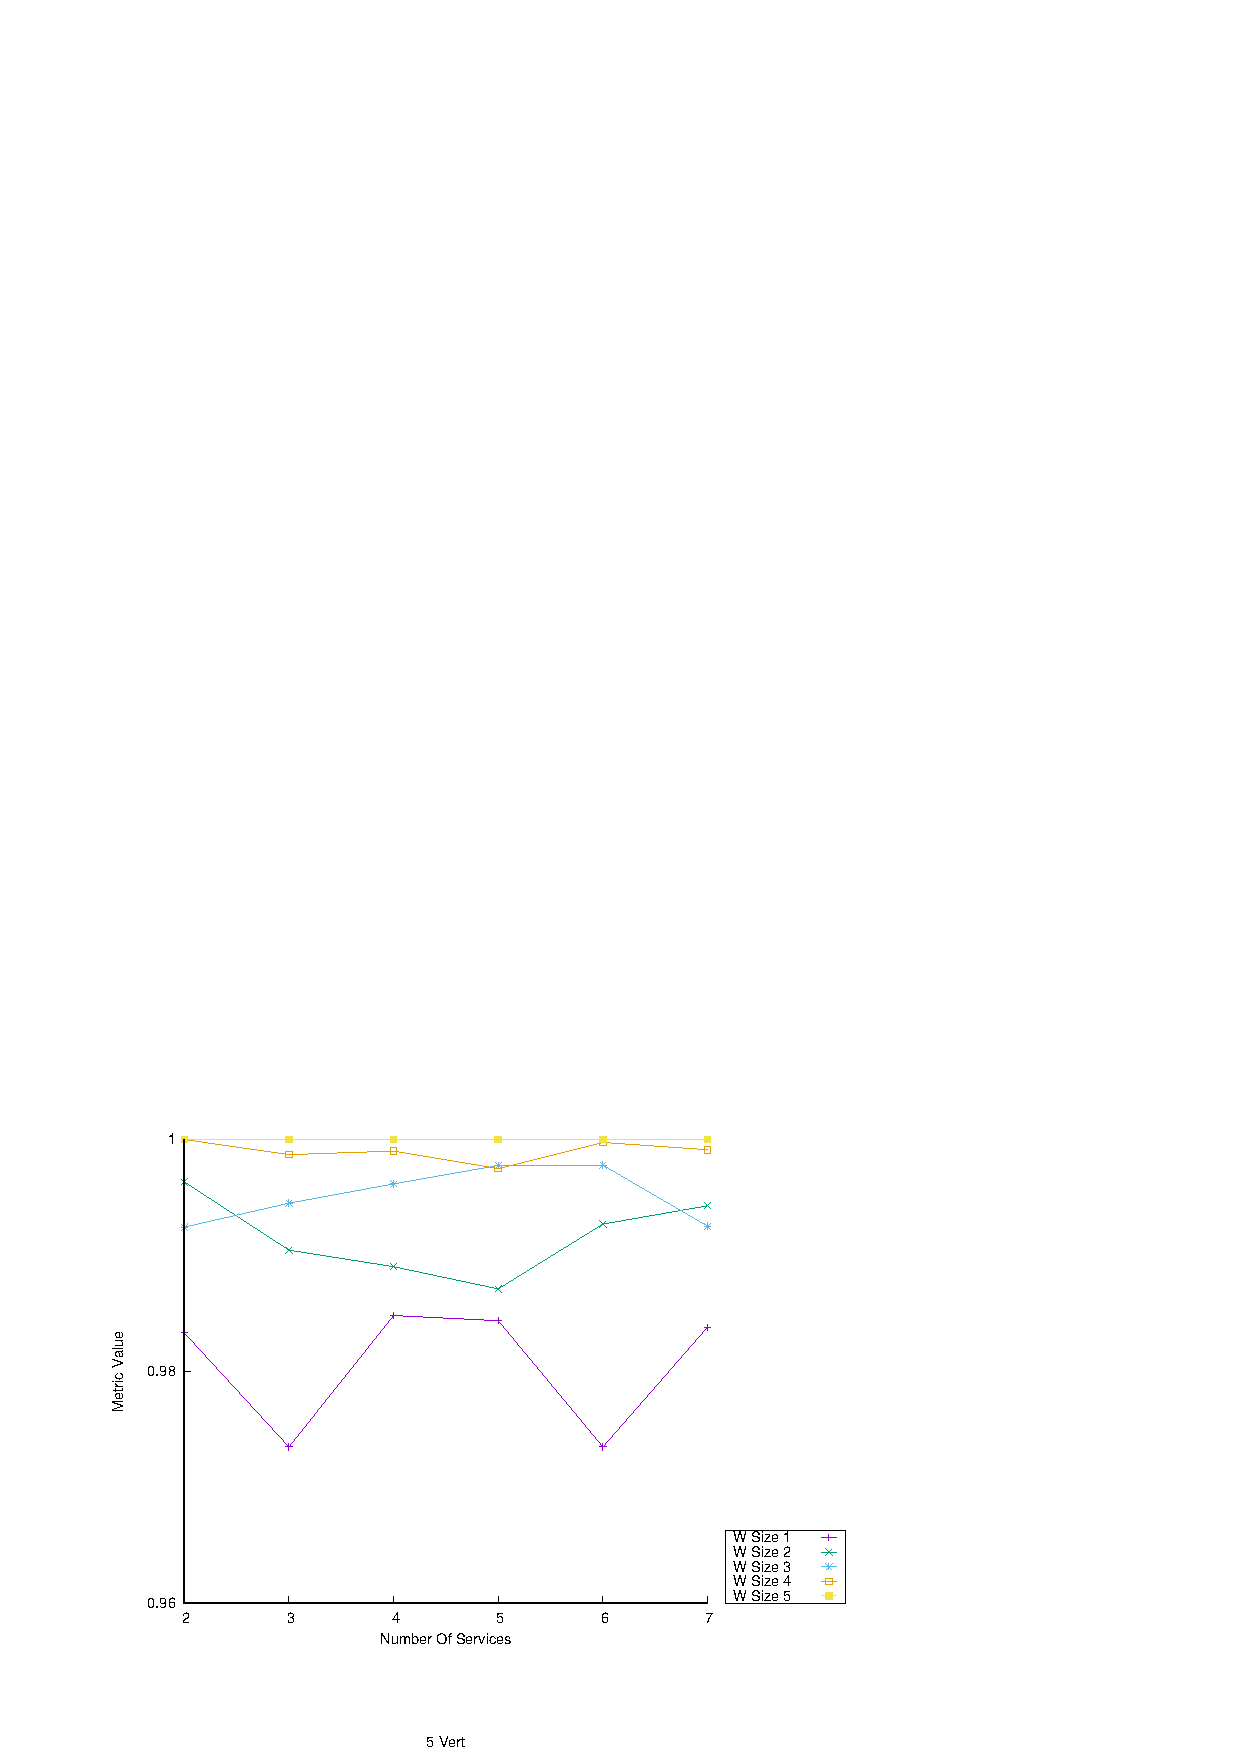
\includegraphics[width=\textwidth]{Images/graphs/window_quality_performance_diff_qual_n7_s7_50_80_n5}
    \caption{5 vertices}
    \label{fig:quality_window_average_qualitative_n5}
  \end{subfigure}
  \hfill
  \begin{subfigure}{0.33\textwidth}
    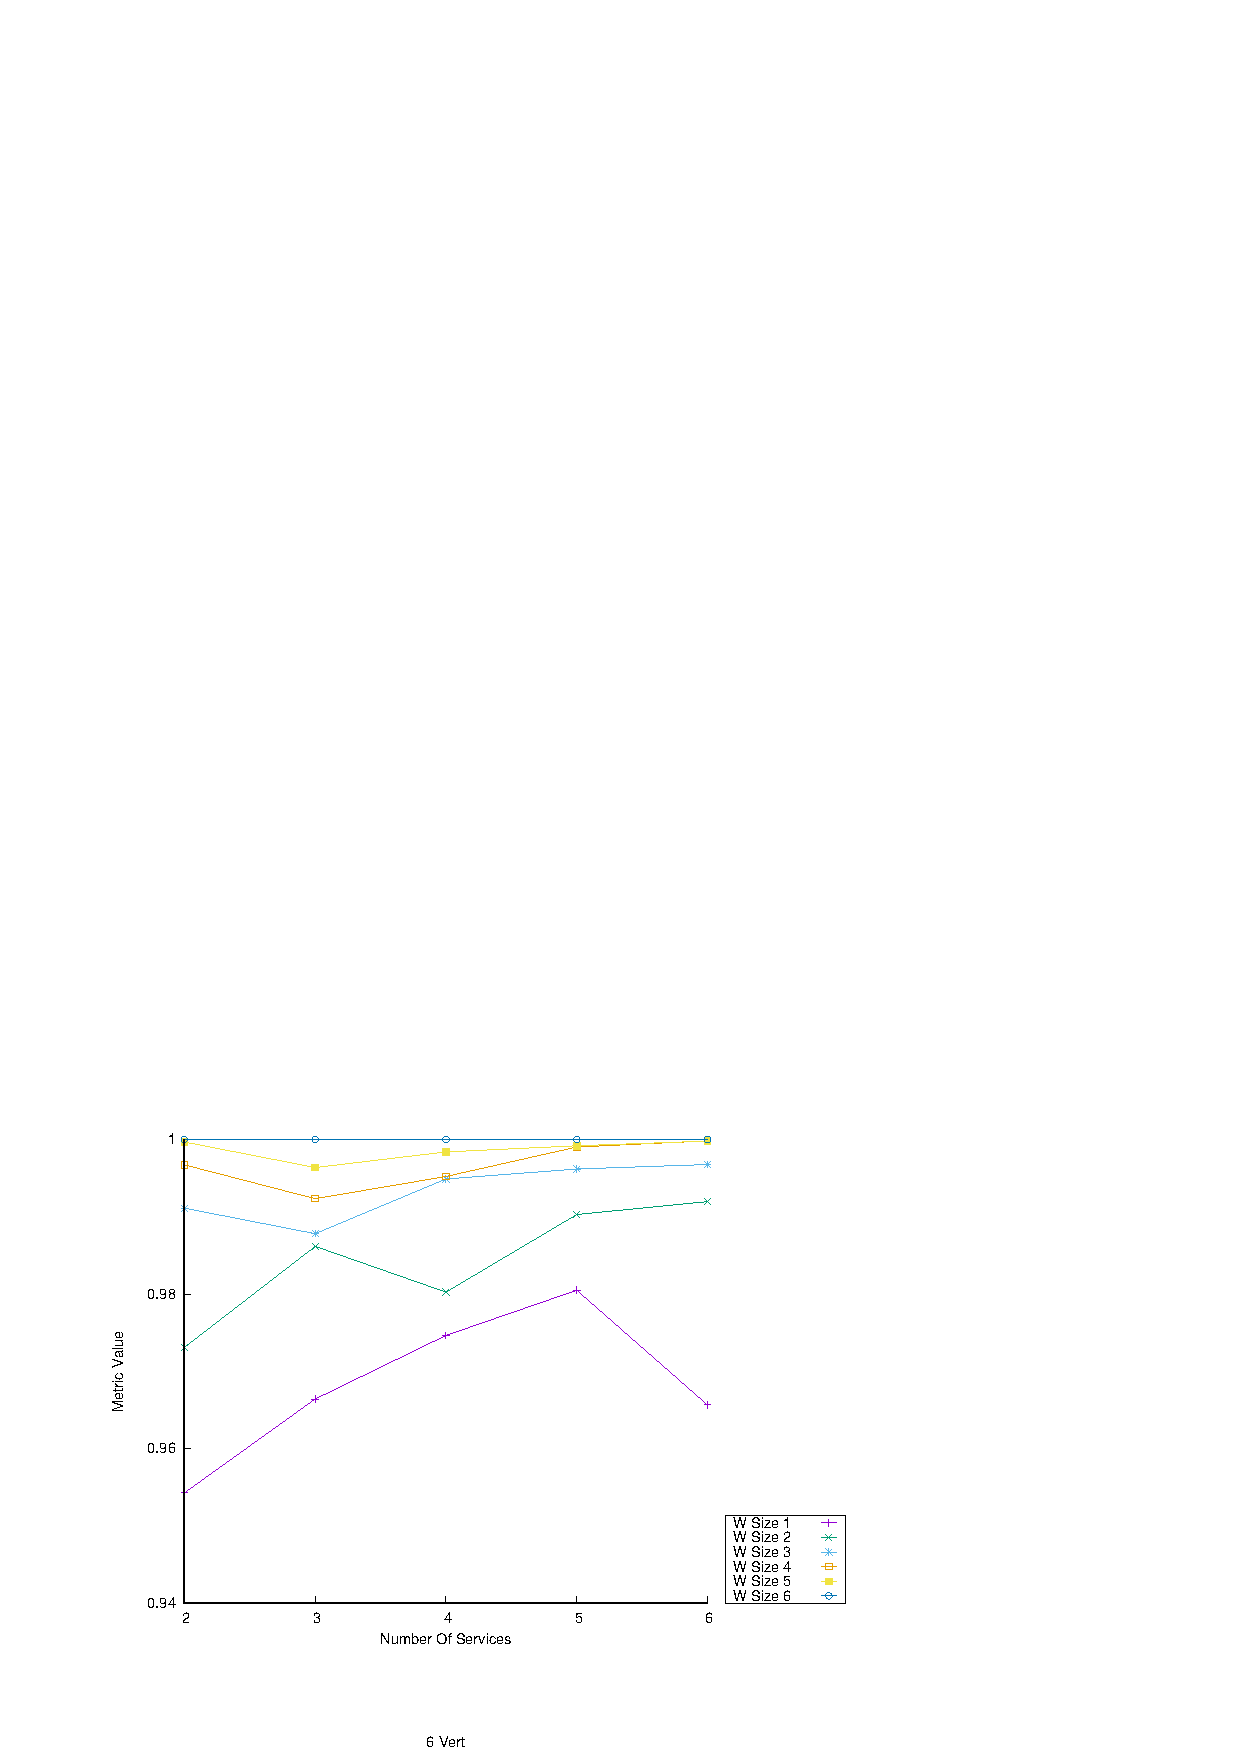
\includegraphics[width=\textwidth]{Images/graphs/window_quality_performance_diff_qual_n7_s7_50_80_n6}
    \caption{6 vertices}
    \label{fig:quality_window_average_qualitative_n6}
  \end{subfigure}
  \begin{subfigure}{0.33\textwidth}
    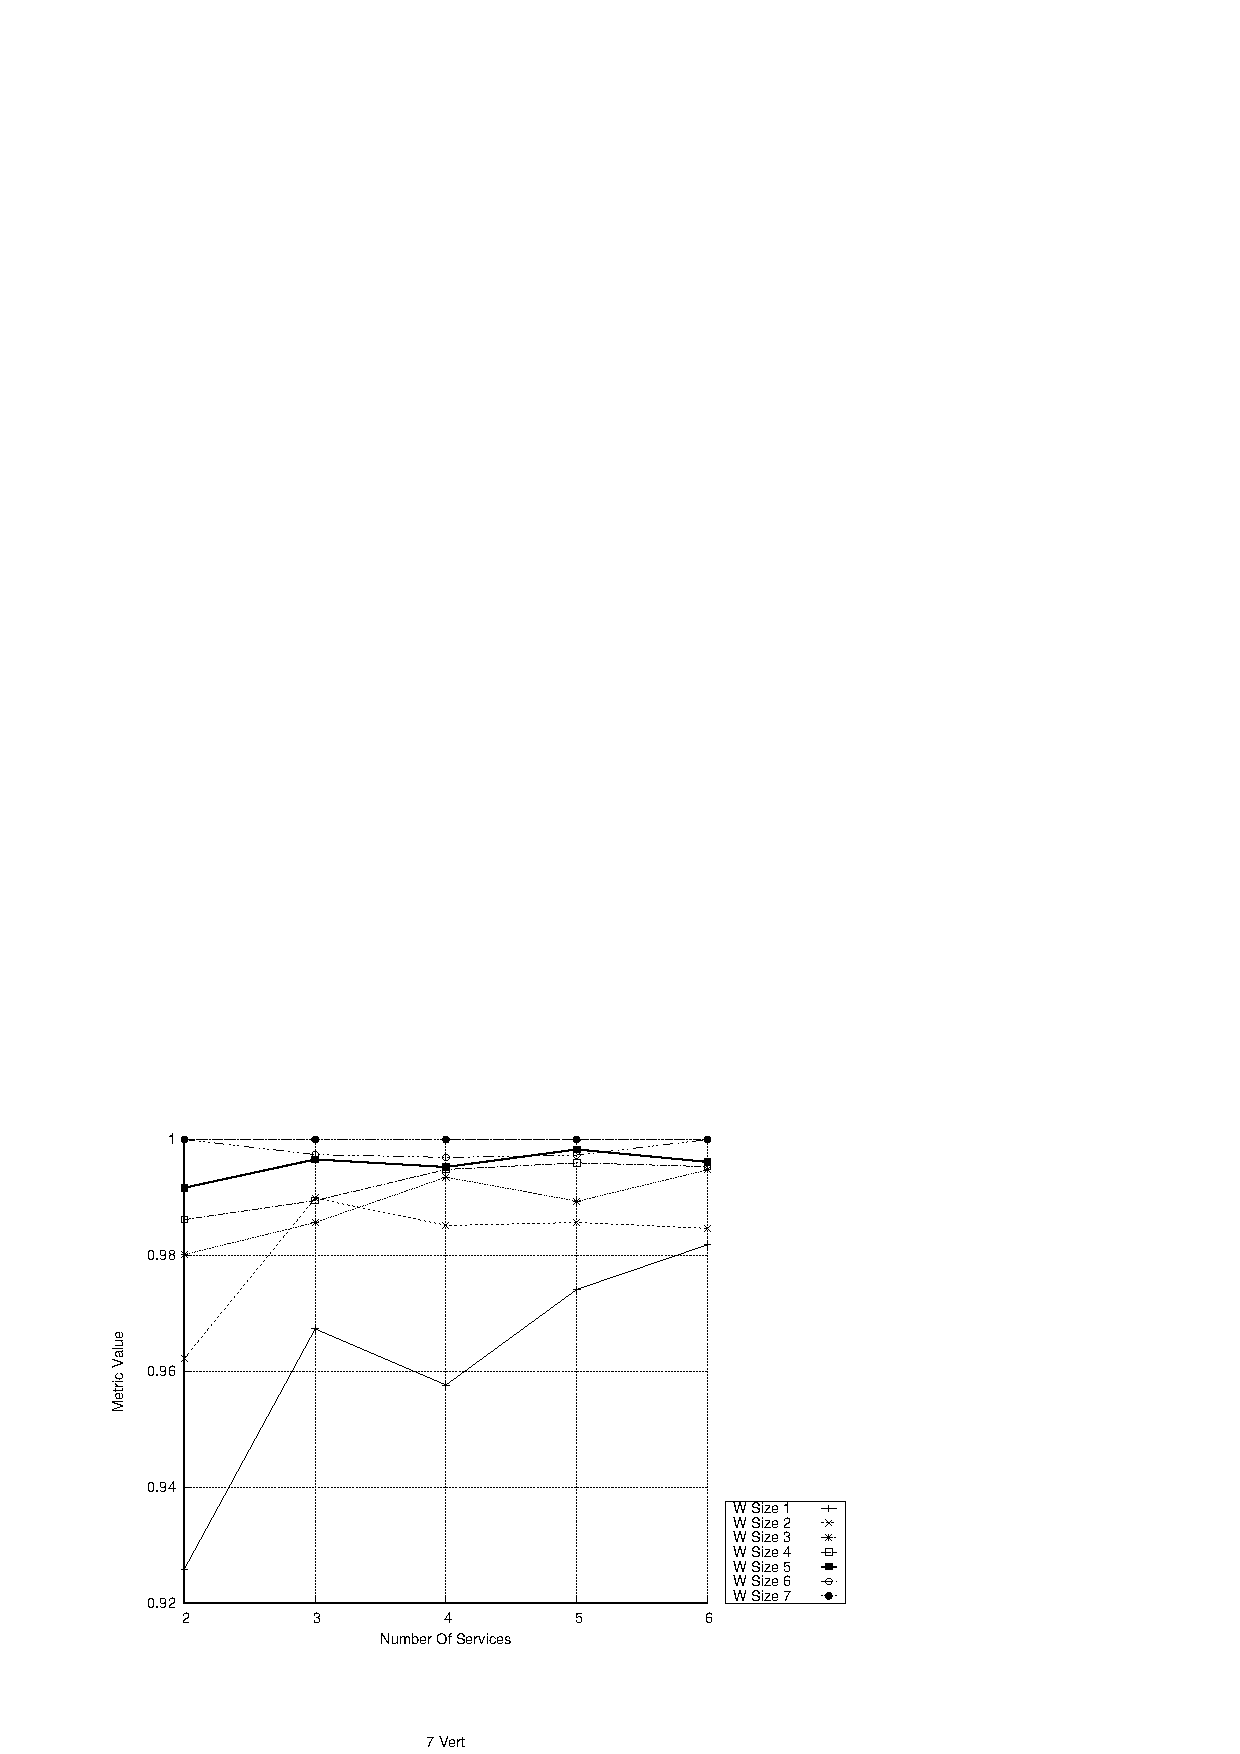
\includegraphics[width=\textwidth]{Images/graphs/window_quality_performance_diff_qual_n7_s7_50_80_n7}
    \caption{7 vertices}
    \label{fig:quality_window_average_qualitative_n7}
  \end{subfigure}

  \caption{Evaluation of Quality Using the \emph{Qualitative} Metric in a \average Profile Configuration.}  \label{fig:quality_window_average_qualitative}
\end{figure*}


